\chapter{Giải pháp hạn chế thiệt hại do thông tin sai lệch gây ra trên mạng xã hội trực tuyến}

Tự do ngôn luận, tự do báo chí là một trong những quyền căn bản của công dân đã được Hiến pháp ghi nhận và đã được Đảng và Nhà nước nhất quán. Tuy nhiên thực tế hiện nay có rất nhiều cá nhân, tổ chức đã và đang lợi dụng các quyền này để xâm phạm lợi ích của Nhà nước và lợi ích chính đáng của công dân. Với sự phát triển mạnh mẽ của Internet và mạng xã hội trực tuyến, việc đăng tải, tuyên truyền các thông tin sai lệch mang tính chất xuyên tạc, chống đối đường lối chính sách của Đảng, pháp luật của Nhà nước, hoạt động của bộ máy chính quyền diễn ra thường xuyên hơn với âm mưu, quy mô và tổ chức ngày càng rộng lớn, chặt chẽ.

Như thường lệ, mỗi khi cơ quan chức năng Việt Nam tiến hành truy tố, xét xử những cá nhân có hành vi vi phạm pháp luật như: Hoạt động nhằm lật đổ chính quyền nhân dân (theo Điều 109 Bộ luật Hình sự năm 2015, sửa đổi bổ sung năm 2017); tuyên truyền chống Nhà nước Cộng hòa XHCN Việt Nam (Điều 117) hay lợi dụng các quyền tự do, dân chủ, xâm phạm lợi ích của Nhà nước, quyền, lợi ích hợp pháp của tổ chức, công dân (Điều 331) thì ngay lập tức một số tổ chức, cá nhân chống đối trong và ngoài nước lại ráo riết tuyên truyền xuyên tạc, chống phá Việt Nam trên lĩnh vực dân chủ, nhân quyền. Những đối tượng này đã lợi dụng quyền tự do ngôn luận để viết và đăng tải các nội dung sai lệch, không có căn cứ, tuyên truyền xuyên tạc đường lối, chính sách của Đảng, pháp luật của Nhà nước, bôi nhọ các cán bộ, Đảng viên làm ảnh hưởng đến uy tín của cơ quan, tổ chức, đi ngược lại với lợi ích quốc gia, dân tộc.

Xuất phát từ những thực tế nêu trên, nhóm tác giả nhận thấy việc nghiên cứu đề ra giải pháp ngăn chặn kịp thời sự lan truyền của thông tin sai lệch trên MXH là một thách thức lớn cần giải quyết kịp thời. Từ thực trạng trên nhóm tác giả đề xuất xây dựng hai bài toán ngăn chặn.

Bài toán đầu tiên với nguồn ngân sách hạn chế, hạn chế bước thời gian lan truyền thông tin, yêu cầu tìm ra $k$ đỉnh có vai trò quan trọng nhất đối với quá trình lan truyền thông tin. Bài toán thứ hai không hạn chế nguồn ngân sách, không hạn chế bước thời gian lan truyền thông tin, yêu cầu tìm tập ít đỉnh nhất đảm bảo số người dùng không bị nhiễm thông tin sai lệch vượt quá một ngưỡng cho trước.

Hai bài toán này đều dựa trên những yêu cầu thực tế, và bản chất của 2 bài toán này là các bài toán tối ưu. Ứng với mỗi bài toán, nhóm tác giả đề xuất một thuật toán (giải pháp) tương ứng để giải quyết, đồng thời chứng minh độ tốt về mặt lý thuyết của thuật toán.

Bên cạnh đó, nhóm tác giả còn đưa ra các kết quả thực nghiệm của hai giải pháp đã được đưa ra đối với hai bài toán tương ứng trên dữ liệu có sẵn, từ đó để thấy được hiệu quả của phương pháp nhóm đề xuất về kết quả và thời gian. Dữ liệu có sẵn là các bộ dữ liệu được lấy từ những nguồn uy tín hàng đầu, được các bài báo có chung mục tiêu nghiên cứu khác sử dụng và được các hội nghị, hội thảo thế giới công nhận. Việc thực nghiệm này sau khi đã kiểm chứng độ tốt về mặt lí thuyết cho thấy các giải pháp mà nhóm tác giả đề xuất có hàm lương học thuật cao, khả thi về mặt lý thuyết.

\section{Bài toán 1: Ngăn chặn thông tin sai lệch với ngân sách giới hạn)}
Bài toán này được đề xuất và nghiên cứu sau khi xem xét thực tế quá trình lan truyền của một thông tin sai lệch trên mạng xã hội. Thông tin sai lệch luôn bắt đầu từ một số người dùng nhất định (có thể coi như đỉnh “nguồn” phát tán thông tin sai lệch). Những người dùng này thường là những kẻ có tư tưởng lệch lạc, phản động, và thông tin sai lệch thường là những thông tin bị bóp méo, những sai lầm của cán bộ bị thổi phồng, hoặc những lời lẽ bịa đặt vô căn cứ. Từ những người dùng bắt đầu này, thông tin sẽ được biết đến bởi những người xung quanh có liên kết với chúng, thường là những người dùng có quan hệ bạn bè với chúng. Thông tin này ban đầu có thể không tác động tới người dùng xung quanh, tuy nhiên nếu nó xuất hiện thêm nhiều lần từ nhiều nguồn khác nhau thì họ có thể sẽ tiếp nhận thông tin đó, và từ đó trở thành một nguồn phát thông tin sai lệch mới. Nếu mọi việc cứ phát triển thì thông tin này dần dần sẽ lan truyền sang toàn bộ một cộng đồng, hoặc thậm chí là toàn MXH (Quá trình lan truyền này được biểu diễn thông qua mô hình lan truyền được định nghĩa bên dưới). Do đó, cần có phương pháp giúp kiểm soát tình hình, ngăn chặn thông tin sai lệch lan truyền quá rộng, và đây cũng là lí do mà giải pháp này được nghiên cứu và công bố. Giải pháp được thiết kế để có thể chọn một số người dùng đặc biệt. Những người dùng được chọn này sau đó sẽ được các cơ quan chức năng có thẩm quyền tiến hành các phương pháp phù hợp đề ngăn chặn khả năng phát tán thông tin của họ. Từ đó, thông tin sai lệch sẽ không có khả năng truyền thông qua những người dùng này, và dẫn đến khả năng lan truyền sang những người dùng tiếp theo bị cản trở. Giải pháp này đã được chứng minh rằng nó có thể lựa chọn ra các đỉnh hiệu quả nhất để ngăn chặn, do đó vừa đem lại hiệu quả cao mà không hao tốn quá nhiều tài nguyên vào việc ngăn chặn các đỉnh kém hiệu quả khác.
	\subsection{Tổng quan bài toán}
	Bài toán này được đưa ra nghiên cứu dựa trên những nhận định về việc thông tin lan truyền trên một mạng xã hội trong thực tế từ người dùng này đến người dùng khác có thể được coi như các bước lan truyền thông tin độc lập diễn ra liên tiếp nhau. Nếu ta càng ngăn chặn được sự lan truyền thông tin sai lệch sớm bao nhiêu, thì hậu quả mà thông tin sai lệch để lại sẽ càng được hạn chế bấy nhiêu. Không chỉ thế, các nghiên cứu gần đây cũng đã chỉ ra rằng số các bước lan truyền thường nhỏ, ví dụ như trong \cite{cha23} đã chỉ ra rằng số các bước lan truyền liên tiếp nhau thông thường chỉ nhỏ hơn 4, và trong \cite{lesk16} một bước lan truyền xảy ra thường là giữa hai người dùng có liên kết trực tiếp với nhau.
	Giải pháp tập trung vào việc tìm ra tập đỉnh $A$ có tối đa $k$ đỉnh để loại bỏ khỏi đồ thị để có thể tối thiểu hóa tác hại của lan truyền thông tin sai lệch. Những khía cạnh mới mà giải pháp của chúng tôi đề ra so với các công trình trước đó là: quá trình lan truyền được giới hạn trong khoảng $d \geq 1$ bước lan truyền bắt đầu từ nguồn phát tán thông tin sai lệch, và giải pháp được thực hiện trên một mô hình lan truyền xác định bởi thực tế cho thấy thông tin cá nhân của người dùng có thể được thu thập qua khảo sát và các phương pháp khai phá dữ liệu \cite{zaixin}. Cụ thể, giải pháp này của chúng tôi có thể được tóm tắt lại như sau:
	\begin{itemize}
		\item Chúng tôi đưa là một mô hình lan truyền thông tin với giới hạn về thời gian lan truyền thông tin, được mở rộng từ mô hình Ngưỡng tuyến tính xác định (Deterministic Linear-Threshold), gọi là mô hình Ngưỡng tuyến tính với bước thời gian rời rạc (Time Constraint Deterministic Linear-Threshold). Sau đó, chúng tôi định nghĩa bài toán Hạn chế sự lây lan của thông tin sai lệch (Limiting the Spread of Epidemics - LSE) với mục tiêu tìm kiếm tập đỉnh $A$ có kích thước tối đa $k$ để loại ra khỏi đồ thị sao cho số đỉnh cứu được là tối đa trong một ràng buộc thời gian. Chúng tôi chỉ ra bài toán này là bài toán NP-Khó và nó không thể xấp xỉ lời giải với tỉ lệ $n^{1-\epsilon}$, $0 < \epsilon < 1$.
		\item Với lời giải, chúng tôi đưa ra Thuật toán nhanh và hiệu quả để giới hạn sự lây nhiễm thông tin (Fast And Effective Limiting Epidemics – FLE).
		\item Việc kiểm thử được thực hiện trên các bộ dữ liệu thực tế lấy từ các nguồn đáng tin cậy như Gnutella, Wikipedia Vote, Amazon và Google Web, đồng thời chúng tôi cũng sử dụng một bộ dữ liệu được thu thập trực tiếp trên Facebook Việt Nam. Thuật toán đã được kiểm nghiệm và cho thấy khả năng ưu việt về cả tốc độ lẫn chất lượng lời giải so với các thuật toán phổ biến được dùng. Chi tiết về kiểm nghiệm sẽ được nêu rõ ở chương sau.
	\end{itemize}  
 	\subsection{Mô hình lan truyền thông tin Ngưỡng tuyến tính với bước thời gian rời rạc (Time Constraint Deterministic Linear Threshold - T-DLT).}
 	Như đã được trình bày ở trên, có hai mô hình phổ biến trong bài toán lan truyền thông tin nói chung là mô hình IC và mô hình LT. Tuy nhiên, ở giải pháp này chúng tôi đề xuất một mở rộng mô hình DLT \cite{zaixin}, vốn cũng là một trường hợp biến thể của mô hình LT, được gọi là T-DLT. Sở dĩ chúng tôi sử dụng mô hình này thay cho mô hình LT và IC bởi với bài toán này, mô hình T-DLT cho phép chúng tôi giảm thiểu tính phức tạp của cơ chế lan truyền, đồng thời vẫn đảm bảo kết quả không bị ảnh hưởng so với hai mô hình điển hình trên. Chi tiết mô hình T-DLT có thể được mô tả như sau:
 	\begin {itemize}
 	\item {\itshape Ký pháp đồ thị}: Đặt $G=(V,E,w)$ là biểu diễn của mạng xã hội với tập đỉnh $V$, tập cạnh có hướng $E$, với $|V|=n$ và $|E|=m$. Mỗi đỉnh đại diện cho một người dùng trong mạng xã hội, mỗi cạnh $e=(u,v)$ trong tập $E$ tương ứng đại diện cho mỗi quan hệ giữa người dùng $u$ và người dùng $v$. Chúng tôi ký hiệu đỉnh vào liền kề và đỉnh ra liền kề của đỉnh $u$ lần lượt là $N_{\textup{in}}(u)$ và $N_{\textup{out}}(u)$, $d_{\textup{in}}(u)$ và $d_{\textup{out}}(u)$ lần lượt là bậc vào và bậc ra của đỉnh $u$. Đặt $I \subset V$ là tập các đỉnh bị lây nhiễm ban đầu. Mỗi cạnh có hướng $(u,v)$ sẽ có trọng số $w(u,v)$, tượng trưng cho mức độ ảnh hưởng thông tin của $v$ tới $u$, thỏa mãn $\sum_{u} w(u,v) \leq 1$.
 	
 	\item {\itshape Trạng thái của đỉnh}: Quá trình phát tán thông tin sai lệch từ tập đỉnh ban đầu $I$ tới các đỉnh còn lại trong mạng xã hội tiến triển theo từng bước thời gian rời rạc $t=1,2,…,d$. Mỗi đỉnh $v \in V$ có hai trạng thái là {\itshape bị lây nhiễm (hay “kích hoạt”)} và {\itshape không bị lây nhiễm (hay “không kích hoạt”)}.
 	
 	\item {\itshape Ngưỡng lây nhiễm (hay ngưỡng kích hoạt)}: Mỗi đỉnh $v$ sẽ có một ngưỡng lây nhiễm cho trước $\theta_{v} \in [0,1]$. Giá trị này đại diện cho trọng số vào của đỉnh $v$ cần chuyển thành bị lây nhiễm để $v$ trở thành bị lây nhiễm.
 	
 	\item {\itshape Quá trình lan truyền}: Quá trình lây lan thông tin sai lệch được mô phỏng tuần tự theo từng bước thời gian rời rạc (còn gọi là “vòng”, “bước”) $t=0,1,2,…,d$. Đặt $I_{t}$ là tập các đỉnh bị lây nhiễm sau $t$ bước, quá trình lan truyền được mô phỏng như sau:
 	\begin {enumerate} [+]
 	\item Tại bước $t=0$, tất cả các đỉnh trong tập $I$ đều bị lây nhiễm, $I_{0}=I$.
 	
 	\item Tại bước $t\geq1$, tất cả các đỉnh không bị lây nhiễm $v$ sẽ chuyển thành bị lây nhiễm nếu tổng trọng số các cạnh vào gần kề chạm ngưỡng lây nhiễm của nó, $\sum_{\text{các đỉnh vào gần kề của $u$}} w(u,v) \geq \theta_{v}$.	
 	
 	\item Một đỉnh bị lây nhiễm sẽ giữ nguyên trạng thái bị lây nhiễm cho tới hết quả trình lan truyền. Qúa trình lan truyền chấm dứt khi $t = d$.
 	\end {enumerate}
 	\end {itemize}
 	Trong mô hình LT, giá trị của ngưỡng $\theta_{v}$ được đặt một cách ngẫu nhiên trong khoảng $[0,1]$ và sẽ được chỉnh sửa dựa vào thông tin có được thêm trong quá trình lan truyền. Do đó, mô hình này thuộc dạng mô hình ngẫu nhiên. Khác với mô hình LT, trong mô hình T-DLT ngưỡng lây nhiễm $\theta_{v}$ được cho trước. Trường hợp này, giá trị ngưỡng có thể được đặt dựa theo các khảo sát thực tế hoặc các phương pháp khai phá dữ liệu.
 	
 	\subsection{Định nghĩa bài toán}
 	Đối với giải pháp này, việc ngăn chặn thông tin sai lệch được tiến hành bằng cách loại bỏ một số người dùng ra khỏi mạng để thông tin không thể truyền qua được, sao cho phạm vi lan truyền của thông tin là nhỏ nhất có thể. Nếu như coi mạng xã hội là một đồ thị, thì ta có thể hiểu rằng những đỉnh “bị lây nhiễm” là những người dùng đã bị ảnh hưởng bởi thông tin sai lệch và thông tin sai lệch đó có thể truyền từ người dùng này sang những người dùng thân cận, những đỉnh “không bị lây nhiễm” là những đỉnh không bị ảnh hưởng bởi thông tin sai lệch, còn những đỉnh “cứu được” là những đỉnh mà có trạng thái chuyển từ “bị lây nhiễm” sang “không bị lây nhiễm” khi chiến thuật loại bỏ đỉnh được áp dụng. Trong thực tế, việc loại bỏ một người dùng ra khỏi mạng xã hội có thể được thực hiện bằng cách thuyết phục người dùng đó thoát khỏi sự ảnh hưởng của thông tin sai lệch, hoặc ngăn chặn kết nối mạng của người dùng đó, hoặc xóa bỏ tài khoản của người dùng ra khỏi mạng xã hội, v.v… Tuy nhiên, những cách làm này đều là những cách làm yêu cầu có sự phối hợp từ nhiều bên liên quan, do đó nếu tiến hành loại bỏ quá nhiều sẽ dẫn đến chi phí phát sinh về thời gian và vật chất rất lớn, thậm chí sẽ gây ra trường hợp loại bỏ thành công như không kịp thời, khiến thông tin lan truyền quá rộng dẫn đến vô ích. Vì vậy, vấn đề đặt ra là phải làm sao chọn ra được một số lượng $k$ đỉnh nào đó để khi thực hiện chiến thuật loại bỏ, ta có được số đỉnh cứu nhiều nhất. Số lượng $k$ sẽ được tính toán một cách cân đối, cẩn thận nhất về chi phí để không làm mất tác dụng của chiến thuật loại bỏ. Chiến thuật loại bỏ $k$ đỉnh này có thể được mô hình hóa và phát biểu khoa học như sau:  
 	
 	Kí hiệu $f_{d}(I)$ là tập hợp các đỉnh đã bị lây nhiễm sau $d$ vòng trên đồ thị $G = (V,E)$ trong mô hình T-DLT, $f_{d}(I,A)$ là tập các đỉnh bị lây nhiễm sau khi loại bỏ một tập các đỉnh $A \subseteq V \setminus I$ từ $G$ (số đỉnh bị lây nhiễm trong đồ thị sót lại). Khi đó, số đỉnh cứu được khi loại bỏ tập $A$ là: $h_{d}(A)=| f_{d}(I,\emptyset)|-|f_{d}(I,A)|$.
 	
 	Trong mô hình T-DLT, ta xây dựng một bài toán tối ưu tổ hợp là: {\itshape Hạn chế sự lây lan của thông tin sai lệch} (Limiting the Spread of Epidemics - LSE), có mục tiêu tìm kiếm một tập đỉnh có kích cỡ tối đa $k$ đỉnh sao cho khi loại bỏ tập đỉnh đó, số đỉnh cứu được sẽ đạt cực đại.  
 	
 	{\itshape Định nghĩa (Bài toán LSE): Cho đồ thị vô hướng $G=(V,E)$ biểu diễn một mạng xã hội trong mô hình T-DLT. Một tập các đỉnh bị lây nhiễm ban đầu $I \subset V$, số vòng lan truyền $d$ và số đỉnh tối đa loại bỏ được là $k > 0$. Tìm một tập $k$ đỉnh  $A \subseteq V \ I$ sao cho khi loại bỏ khỏi mạng thì số đỉnh cứu được sau $d$ vòng là $h_{d}(A)$ đạt cực đại.}
 	
 	Kí hiệu $G_{d} = (V_{d}, E_{d})$ đồ thị con của đồ thị $G=(V, E)$ trong đó $V_{d}$ là tập các đỉnh mà khoảng cách giữa một đỉnh bất kì trong đó với một đỉnh trong tập $I$ tối đa là $d$, và tập $E_{d}$ là tập các cạnh nối giữa các đỉnh thuộc tập $V_{d}$, đồng thời $n_{d} = | V_{d} |$, $m_{d} = | E_{d} |$. Ta thấy rằng sự lan truyền thông tin sai lệch chỉ xảy ra bên trong đồ thị con $G_{d}$. Do đó, để đơn giản hóa, thay vì xét đến tất cả các đỉnh thuộc $G$, ta sẽ chỉ tìm kiếm kết quả trong đồ thị con $G_{d}$.
 	
 	\subsection{Độ phức tạp và tính xấp xỉ của bài toán LSE}
 	Trong mục này, chúng tôi chỉ ra tính NP-Khó của bài toán LSE bằng cách tương đương hóa bài toán LSE với bài toán Phủ đỉnh (Set Cover). Chúng tôi cũng sẽ chỉ ra tính khó xấp xỉ của LSE, tức là việc xấp xỉ bài toán LSE với tỉ lệ $n^{1 - \varepsilon}$, với $0 < \varepsilon < 1$, là bài toán NP-Khó.
 	
 	{\itshape Định lí: LSE là bài toán NP-Khó trong mô hình T-DLT}.
 	
 	{\itshape Chứng minh:} Để chứng minh LSE là bài toán NP-Khó, ta giản thể bài toán về bài toán Phủ đỉnh (Set cover) 
 	
 	{\bfseries Bài toán Phủ đỉnh (Set Cover - SC):} Cho một số tự nhiên dương $t$, một tập phổ quát $\vartheta = {e_{1}, e_{2}, ... ,e_{M}}$ và tập con $S = {s_{1}, s_{2}, ... , s_{N}}$ ta có thể giả sử rằng $t < M < N$. Bài toán Phủ đỉnh yêu cầu rằng: Có tồn tại hay không một lượng $t$ tập con, sao cho hợp của chúng là $\vartheta$.
 	
 	Bài toán SC đã được chứng minh là bài toán NP-Khó khi kích thước các tập được giới hạn là 3 và mỗi phần tử xuất hiện trong đúng hai tập con. Để giản thể bài toán SC về bài toán LSE, đầu tiên chúng tôi xây dựng một biểu diễn $J_{\text{LSE}}$ của bài toán LSE từ biểu diễn $J_{\text{SC}}$ của bài toán SC. Sau đó chúng tôi chỉ ra rằng nếu $J_{\text{SC}}$ có tồn tại lời giải $S$ kích thước $t$, thì $J_{\text{LSE}}$ có lời giải $A$, $| A | \leq k$ với $h_{d}(A) \geq k + M$ và ngược lại.
 	
 	{\bfseries Xây dựng:} Cho một biểu diễn $J_{SC} = (\vartheta, S, t)$ của bài toán SC, ta xây dựng biểu diễn $J_{LSE} = (G, I, d, k)$ của bài toán LSE như theo hình \ref{refhinh3_3}
 	\begin {itemize}
 	\item {\itshape Tập các đỉnh và các cạnh}: với mỗi $S_{i} \in S$, ta xây dựng một đỉnh bị lây nhiễm ban đầu $s_{i} \in I$ và một đỉnh $u_{i}$. Ta có thêm một cạnh có hướng $(s_{i}, u_{i})$. Với mỗi phần tử $e_{j} \in \vartheta$ ta thêm một đỉnh $v_{j}$ và thêm một cạnh có hướng $(u_{i},v_{j})$ với mỗi $u_{i}$. Để thuận tiện, ta đặt $B = {u_{1}, u_{2}, ... , u_{N}}$, $C = {v_{1}, v_{2}, ... , v_{M}}$.
 	
 	\item {\itshape Ngưỡng lây nhiễm và trọng số}: ta đặt $w(u,v) = 1$,\linebreak $w(u_{i}, v_{i}) = \dfrac{1}{d_{in}(v_{j})}$, $\theta_{u_{i}} = \theta_{v_{i}} = 1$.
 	
 	\item Sau cùng, ta cho $k = t$, $d = 2$. 		
 	
 	\begin{center}
 		\begin{figure}[H]
 			\begin{center}
 				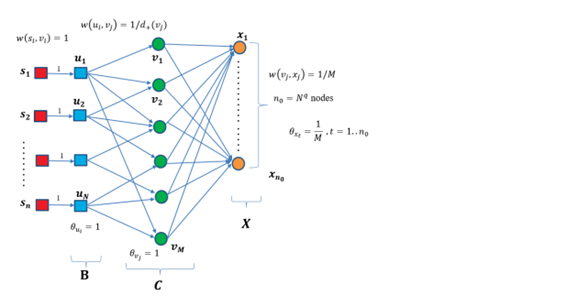
\includegraphics [scale=1]{picture/Hinh3_3}
 			\end{center}
 			\caption{Giản thể từ bài toán SC về bài toán LSE.}
 			\label{refhinh3_3}
 		\end{figure}
 	\end{center}
 	\end {itemize}
 	{\bfseries Phân tích:} Qua bước xây dựng, ta thấy rằng $| f_{d}(I,\emptyset) | = M + N$. Nếu như có đỉnh bất kì $u_{i} \in B$ là đỉnh kề vào và $v_{j} \in C$ là đỉnh chưa bị lây nhiễm thì: 
 	\begin{center}
 		$\sum_{\text{Các đỉnh hàng xóm tới đã bị lây nhiễm $u$}} w(u, v_{j}) \leq 1 - \dfrac{1}{d_{in}(v_{j})} < 1 = \theta_{v_{j}}$.
 	\end{center}
 	
 	Do đó $v_{j}$ lầ đỉnh không bị lây nhiễm. Nếu không, các đỉnh trong $C$ là các đỉnh không bị lây nhiễm.
 	
 	($\rightarrow$) Giả sử $S'$ là lời giải của biểu diễn $J_{\text{SC}}$, có nghĩa là $| S' | = t = k$ và nó phủ $t$ phần tử của $\vartheta$. Nếu ta chọn tập $A$ chứa đỉnh $u_{i}$ tương ứng với $S_{i} \in S'$, với mọi đỉnh $v_{i} \in B$ kề với ít nhất một đỉnh trong $A$. Bằng bước phân tích trên, mọi đỉnh trong $C$ là đỉnh không bị lây nhiễm. Ta có $h_{d}(A) = t + M = k + M$.
 	
 	($\leftarrow$) Ngược lại, nếu $J_{\text{LSE}}$ có lời giải $A$, $|A| \leq k$ với $h_{d}(I, A) \geq k + M$. Nếu $A$ chứa $t_{1} (1 \leq t_{1} \leq k)$ đỉnh trong $C$, $h_{d}(I, A) \leq k - t_{1} + M < k + M$. Do đó $A$ không chứa bất kì đỉnh nào thuộc $C$. Ở đây, $A \subset B$. Kết hợp với $h_{d}(I, A) \geq k + M$, mọi đỉnh thuộc $C$ là đỉnh không bị lây nhiễm. Do đó, mọi đỉnh $u_{i} \in A$ kề ít nhất với một đỉnh thuộc $C$. Vì vậy, qua bước xây dựng ta thấy rằng, $S' = \{ S_{i} | u_{i} \in A \}$ là lời giải cho bài toán $J_{\text{SC}}$. Định lý được chứng minh.
 	
 	Bằng cách thay đổi một chút phương pháp chứng minh bên trên, ta có thể chứng minh thêm được một định lý về tính khó xấp xỉ của bài toán LSE.
 	
 	Định lý: Đánh giá xấp xỉ bài toán LSE với tỉ lệ $n^{1 - \varepsilon}$ trong mô hình T-DLT với mọi hằng số $0 < \varepsilon < 1$ là bài toán NP-khó .
 	
 	{\itshape Chứng minh}: Để chứng minh kết quả này, ta sử dụng phương pháp {\itshape gap-introduction reduction} \cite{vijay38} để chứng minh tính khó xấp xỉ của bài toán LSE. Sử dụng phép giản thể trong thời gian đa thức thành bài toán SC từ bài toán LSE , chúng tôi sẽ chỉ ra nếu tồn tại một thuật toán có thời gian đa thức có thể xấp xỉ được bài toán trên với tỉ lệ $n^{1 - \varepsilon}$, thì sẽ tồn tại một thuật toán có thời gian đa thức để giải bài toán gốc.
 	
 	{\bfseries Xây dựng:} Cho một biểu diễn của bài toán SC, $J_{\text{SC}} = (\vartheta, S, t)$, ta xây dựng một biểu diễn $J_{\text{LSE}} = (G, I, d, k)$ 
 	\begin {itemize}
 	\item {\itshape Tập các đỉnh và các cạnh}: Với mỗi đỉnh $v_{j} \in C$, ta thêm $n_{0} = N^{q}$ đỉnh $X = { x_{1}, x_{2}, ... , x_{n_{0}}}$ với một hằng số $q$ đủ lớn và thêm một cạnh có hướng $(v_{j}, x_{l}), l = 1 ... n_{0}$.
 	
 	\item {\itshape Ngưỡng lây nhiễm và trọng số}: Gán $w(v_{j}, x_{l}) = \dfrac{1}{M}$; $\theta_{x_{l}} = \dfrac{1}{M}$, $l = 1 ... n_{0}$.\\
 	\end {itemize}
 	Giả sử $J_{\text{SC}}$ có tập phủ đinh $S'$ kích cỡ $t$, ta chọn tập $A = \{{u_{i} | S_{i} \in S}\}$. Qua bước phân tích ở trên, mọi đỉnh $C$ đều là đỉnh không bị lây nhiễm. Điều này dẫn tới mọi đỉnh trong $X$ đều là các đỉnh không bị lây nhiễm. Bởi bước xây dựng này, ta có: $| f_{d}(I, \emptyset) | = N + M + N^{q}$, $| f_{d}(I, A) | = N - k$, do đó: 
 	\begin{center}
 		$h(A) = | f_{d}(I, \emptyset) | - | f_{d}(I, A) | = M + N^{q} + k$.
 	\end{center}
 	
 	Trong trường hợp $J_{\text{SC}}$ không có tập phủ đỉnh kích thước $t$, nó có ít nhất một đỉnh $v_{j}$ bị lây nhiễm. Điều này dẫn tới việc mọi trong $X$ đều bị lây nhiễm. Do đó, $| f_{d}(I, A) | > N - k + N_{q}$ dẫn tới $h(A) = M  + k < 2N$.
 	
 	Lúc này, giả sử ta có thuật toán thời gian đa thức $ \mathcal{A} $ có thể xấp xỉ bài toán LSE trong tỉ lệ $n^{1 - \varepsilon}$, ta chứng minh rằng lời giải của bài toán SC có thể được tìm trong thời gian đa thức. Với bất kì biểu diễn $J_{\text{SC}}$ nào, ta có thể xây dựng một biểu diễn $J_{\text{LSE}}$ theo cách xây dựng trên trong thời gian đa thức của $m$ và $n$. 
 	
 	Trong trường hợp $J_{\text{SC}}$ có tập đỉnh phủ kích cỡ $t$, theo cách xây dựng của chúng tôi, lời giải tối ưu $A_{\text{opt}}$ của $J_{\text{LSE}}$ có $h(A_{\text{opt}}) = k + M + N_{q}$. Thuật toán $\mathcal{A}$ xấp xỉ lời giải tối ưu với tỉ lệ $n^{1 - \varepsilon}$ ($n = 2N + M + N_{q}$ là số đỉnh của đồ thị đầu vào) do đó có thể tìm kiếm được lời giải $\mathcal{A}(J_{\text{LSE}})$. 
 	\begin{center}
 		$h(\mathcal{A}(J_{\text{LSE}})) \geq \dfrac{1}{n_{1 - \varepsilon}} h(A_{\text{opt}}) > \dfrac{1}{n^{1 - \varepsilon}}(M + N_{q} +k) = \dfrac{n^{\varepsilon}}{n}(M + N^{q} +k) \linebreak > \dfrac{(M + N^{q} + k)^{\varepsilon}}{M + N^{q} + k}N^{q}> \dfrac{N^{q.\varepsilon}}{4N^{q}}N^{q} = \dfrac{1}{4}N^{q.\varepsilon}$. 	
 	\end{center}
 	
 	Cho $q$ đủ lớn để $q > \dfrac{ln(8N)}{\varepsilon.ln(N)}$, ta được: 
 	\begin{center}
 		$h(\mathcal{A}(J_{\text{LSE}})) > 2N$.
 	\end{center}
 	
 	Nếu $J_{\text{LSE}}$ không có tập phủ đỉnh kích cỡ $t$, thì tập tối ưu $A_{\text{opt}}$ của $J_{\text{LSE}}$ có 
 	\begin{center}
 		$h(\mathcal{A}(J_{\text{LSE}})) < 2N$.
 	\end{center}
 	
 	Điều này cho thấy $J_{\text{SC}}$ có một tập phủ đỉnh kích cỡ $t$ khi và chỉ khi $h(\mathcal{A}(J_{\text{LSE}})) < 2N$. Do đó ta có thể dùng $\mathcal{A}$ để giải quyết bài toán SC trong thời gian đa thức, hay $\text{P} = \text{NP}$. Điều này mâu thuẫn với giả thiết $\text{P} \neq \text{NP}$.
 	
 	\subsection{Thuật toán đề xuất}
 	Trong phần này, chúng tôi thiết kế một thuật toán heuristics có độ phức tạp thấp và kết quả rất khả quan. Tên gọi của thuật toán là Thuật toán nhanh và hiệu quả để giới hạn sự lây nhiễm thông tin(Fast And Effective Limiting Epidemics – FLE). 
 	Trước khi bắt đầu, chúng tôi có định nghĩa một vài kí hiệu sẽ được sử dụng trong quá trình đề xuất thuật toán:
 	\begin {itemize}
 	\item $t(u)$: vòng nhỏ nhất sao cho đỉnh $u$ chuyển từ đỉnh không bị lây nhiễm sang đỉnh bị lây nhiễm.
 	
 	\item $a_{\text{in}}(u) = \sum_{I_{t(u) - 1} \bigcap N_{in}(u)} w(u,v):$ tổng trọng số các cạnh vào từ các đỉnh vào hàng xóm đã bị lây nhiễm trước vòng $t(u)$.
 	
 	\item $\alpha(u) = \sum_{v \in U^{d}_{i=t(u)+1}} I_{i} \bigcap N(u)$ $w(u,v), i = t(u) + 1, ... , d$: tổng trọng số các cạnh ra từ $u$ tới các đỉnh bị lây nhiễm $v$ tại vòng $i$.
 	
 	\item $\beta(u): $ : số lượng các đỉnh ra cứu được, sao cho chúng chuyển từ bị lây nhiễm thành không bị lây nhiễm sau khi loại bỏ đỉnh $u$ ra khỏi đồ thị.
 	\end {itemize}
 	 	\begin{algorithm}[H]
 		\caption{Fast Limit Epidemics (FLE) algorithm.}
 		\label{alg:Algo1}
 		%\SetAlgoNlRelativeSize{0}
 		\KwData{Graph $G=(V,E,\emptyset)$, set of initial infected nodes $I$, propagation hop $d$.}
 		\KwResult{Set of nodes $A$}
 		$S \gets \emptyset$; 
 		\\
 		Calculate $G' \gets G_{d}(I); U \gets V_{d}$
 		\\
 		\For {$i=1$ to $k$}
 		{
 			Calculate $\alpha(u)$, $\beta(u)$ on $G'$ (Algorithm 3)
 			\\
 			$u_{\text{max}} \gets 0$
 			\\
 			\eIf {$\beta(v)=0, \forall u \in U$}
 			{
 				$u_{\text{max}} \gets \text{arg max}_{v \in U}\alpha(v)$
 			}
 			{
 				$u_{\text{max}} \gets \text{arg max}_{v \in U}\beta(v)$
 			}
 			$S \gets S \cup \{u_{\text{max}}\}$
 			\\
 			$U \gets U \setminus \{u_{\text{max}}\}$
 			\\
 			Remove $u_{\text{max}}$ and all edges that adjacent with $u_{\text{max}}$ from $G'$
 		}
 		\Return $S$
 	\end{algorithm}
  	
 	Một cách trực quan, số lượng gia tăng các đỉnh được cứu $\delta(A, u)$ có thể xấp xỉ theo $\beta(u)$. Bên cạnh đó, để tăng cường tính hiệu quả của thuật toán đề xuất, chúng tôi kết hợp $\alpha(u)$ và $\beta(u)$ để tính toán khả năng lan truyền tin sai lệch của đỉnh $u$. Ý tưởng chính của thuật toán là chọn ra các đỉnh một cách lần lượt theo đánh giá của hai hàm $\alpha$ và $\beta$. Ban đầu, chúng tôi khởi tạo tập đỉnh được chọn $A=\emptyset$ và đặt tập các đỉnh được xét chọn $U$ bằng với $V_{d}$. Trong mỗi bước, chúng tôi chọn ra đỉnh có trị số $\beta(u)$ lớn nhất trong đồ thị còn lại. Trường hợp tất cả các đỉnh đều có giá trị $\beta(u)$ là 0, chúng tôi chọn đỉnh có giá trị $\alpha(u)$ cực đại. Chi tiết thuật toán được mô tả trong Thuật toán \ref{alg:Algo1}.
 	
 	Khó khăn trong thuật toán chủ yếu đến từ bước tính toán các hàm $\alpha$ và $\beta$. Để giải quyết việc này, chúng tôi bắt đầu với ý tưởng tìm kiếm theo chiều rộng (Breath First Search - BFS) để tính toán $f_{d}(I)$ và dần dần cập nhật hàm $\alpha_{\text{in}}()$. Sau đó, chúng tôi sử dụng nó để tính toán các hàm  $\alpha()$ và $\beta()$ theo định nghĩa của chúng. Chi tiết thuật toán được thể hiện trong Thuật toán \ref{alg:Algo2} và Thuật toán \ref{alg:Algo3}.
 	\begin{algorithm}[hpt]
 		\caption{Calculate $f_{d}(I), a_{\text{in}}(), t()$}
 		\label{alg:Algo2}
 		\KwData{Graph $G=(V,E,\emptyset)$, set of infected nodes $I$, propagation hop $d$.}
 		\KwResult{$f_{d}(I), a_{\text{in}}(u), t(u), \forall u \in G$.}
 		\ForEach {$u$ \textbf{in} $G$}
 		{
 			$t(u) \gets +\infty; a_{\text{in}}(u) \gets 0; \alpha(u) \gets 0; \beta(u) \gets 0$
 		}
 		\ForEach {$s$ \textbf{in} $I$}
 		{
 			$t(s) \gets 0$
 		} 
 		Queue $Q \gets \emptyset$
 		\\
 		\While{$Q \neq \emptyset$}
 		{
 			$u \gets Q.pop()$
 			\\
 			$f_{d}(I) \gets u$
 			\\
 			\If{$t(u)<d$}
 			{
 				\ForEach{$v \in N_{\text{out}}(u)$}
 				{
 					\If{$t(u)<t(v)$}
 					{
 						$a_{\text{in}}(v)=a_{\text{in}}(v)+w(u,v)$
 						\\
 						\If{$a_{\text{in}}(v) \geq \theta_{v}$ \textbf{and} $t(u)+1<t(v)$}
 						{
 							$t(v) \gets t(u)+1$
 							\\
 							$Q,push(v)$
 						}
 					}
 				}
 			}	
 		}
 	\end{algorithm}
 	
 	\begin{algorithm}[hpt]
 		\caption{Calculate $\alpha()$ and $\beta()$}
 		\label{alg:Algo3}
 		\KwData{Graph $G=(V,E,\emptyset)$, set of infected nodes $I$, propagation hop $d$, $f_{d}(I), a_{\text{in}}(), t()$.}
 		\KwResult{$\alpha(u), \beta(u), \forall u \in G$.}
 		\ForEach{$u$ \textbf{in} $f_{d}(I)$}
 		{
 			$\alpha(u) \gets 0; \beta(u) \gets 0$
 			\\
 			\ForEach{$v$ \textbf{in} $N_{\text{out}}(u) \cap f_{d}(I)$}
 			{
 				\If{$t(u)<t(v)$}
 				{
 					$\alpha(u) \gets \alpha(u)+w(u,v)$
 					\\
 					\If{$a_{\text{in}}(v)-w(u,v)<\theta_{v}$}
 					{
 						$\beta(u) \gets \beta(u)+1$
 					}
 				}
 			}
 		}
 	\end{algorithm}
 	
 	{\itshape Chứng minh}: Để đánh giá độ phức tạp của thuật toán này, chúng ta cần đánh giá trước độ phức tạp của thuật toán. Ta dễ thấy rằng việc tính  toán $f_{d}(I)$ (Thuật toán \ref{alg:Algo2}, dòng 7 - 22) có cách thức hoạt đông giống BFS. Do đó, độ phức tạp của nó là $O(m_{d} + n_{d})$. Với bước tính toán $\alpha(u)$ và $\beta(u)$ (Thuật toán \ref{alg:Algo3}, dòng 1 - 11), ta thấy độ phức tạp của nó là $O(m_{d} + n_{d})$. Do đó, độ phức tạp chung của thuật toán là $O(m_{d} + n_{d})$. 
		
\subsection{Kết quả thực nghiệm với dữ liệu có sẵn}

Trong phần này, chúng tôi thực nghiệm thuật toán đối với dữ liệu sẵn có trên một số mạng xã hội trực tuyến để kiểm chứng tính hiệu quả của thuật toán khi so sánh nó với các thuật toán cơ sở được sử dụng trong các bài toán lan truyền thông tin \cite{nguyen30}, \cite{kemple1}, \cite{zhang32}. Chúng tôi so sánh đánh gia trên ba yêu tố chính: chất lượng lời giải, tính mở rộng, tác động của số vòng lan truyền $d$ trên một vài các mạng xã hội trực tuyến thực tiễn. Các thuật toán cơ sở sẽ sử dụng bao gồm:
\begin{itemize}
	\item Random: Thuật toán chọn ngẫu nhiên $k$ đỉnh trong $N_{d}(S)$.
	
	\item Maxdegree (Maxdeg): Thuật toán heuristic chọn lần lượt các đỉnh có bậc cao nhất trong tập $V_{d}$ cho đến khi đủ $k$ đỉnh.
	
	\item Greedy: Thuật toán heuristic chọn lần lượt $k$ đỉnh, trong mỗi lần chọn sẽ chọn ra đỉnh sao cho khi loại bỏ đỉnh đó sẽ cứu được nhiều đỉnh nhất có thể.
\end{itemize}

Chúng tôi thực nghiệm sử dụng một hệ thống máy có cấu hình sau: Intel(R) Core(TM) i5-6200U CPU @ 2.30 GHz (up to 2.40 GHz), bộ nhớ RAM 4GB, ngôn ngữ lập trình Python 2.7.

\subsubsection{Dữ liêu:}

Chúng tôi thực nghiệm thuật toán trên nhiều bộ dữ liệu thực tế khác nhau. Bên cạnh việc lựa chọn các bộ dữ liệu để đảm bảo sự đa dạng về kích thước, chúng tôi cũng lựa chọn nhiều miền dữ liệu khác nhau, bảng \ref{tab:Table1} thể hiện các bộ dữ liệu nhóm tác giả sử dụng.
\begin{table}
	\centering
	\begin{tabular}{|c|c|c|c|c|}
		\hline 
		Mạng & Số đỉnh & Số cạnh & Loại & Bậc trung bình \\ 
		\hline 
		Gnutella & 6,301 & 20,777 & Có hướng & 3.29 \\ 
		\hline 
		Wikipedia vote & 7,115 & 103,689 & Có hướng & 14.57 \\ 
		\hline 
		Amazon & 262,111 & 1,234,877 & Có hướng & 4.71 \\ 
		\hline 
		Google web & 875,713 & 5,105,039 & Có hướng & 5.83 \\ 
		\hline 
	\end{tabular} 
	\caption{Các bộ dữ liệu}
	\label{tab:Table1}
\end{table}

\subsubsection{Các thiết lập}
Chúng tôi sử dụng các thiết lập dưới đây cho việc đánh giá thực nghiệm:

\begin{itemize}
	\item Trọng số của cạnh: $w(u,v)=\frac{1}{d_{\text{in}}(v)}$, với $d_{\text{in}}(v)$ là bậc vào của đỉnh $v$ \cite{kemple1} \cite{chen10LT} \cite{khali} \cite{amit21}.
	\item Ngưỡng lây nhiễm: chúng tôi lựa chọn ngưỡng lây nhiễm trong tập \\ $\{0.1, 0.2, 0.3, 0.4, 0.5, 0.6, 0.7, 0.8, 0.9\}$.
	\item Số vòng lây nhiễm: chúng tôi lựa chọn số vòng lây nhiễm $d = 2, 3, 4, 5$ dựa theo một nghiên cứu có trước \cite{cha23}.
	\item Số đỉnh bị nhiễm ban đầu: trong mọi bộ dữ liệu, chúng tôi lấy $1\%$ số đỉnh làm tập đỉnh bị lây nhiễm ban đầu. 
\end{itemize}

\subsubsection{Các thuật toán sử dụng}
Chúng tôi sử dụng các thuật toán sau đây cho việc đánh giá thực nghiệm cùng với thuật toán FLE, các thuật toán này đều là các thuật toán được nhiều bài báo khác sử dụng trong quá trình đánh giá của mình:

\begin{itemize}
	\item {\itshape Random}: Thuật toán lựa chọn ngẫu nhiên $k$ đỉnh trong đồ thị mạng xã hội để loại bỏ.
	\item {\itshape Greedy}: Thuật toán thực hiện $k$ lần, mỗi lần chạy thuật toán sẽ thử loại bỏ lần lượt từng đỉnh ra khỏi đồ thị và đánh giá số lượng đỉnh cứu được tuong ứng, qua đó lựa chọn ra đỉnh loại đi mà cứu được nhiều đỉnh nhất để loại bỏ.
	\item {\itshape MaxDegree}: Thuật toán thực hiện $k$ lần, mỗi lần chọn thuật toán sẽ chọn ra đỉnh có bậc lớn nhất để loại nó ra khỏi đồ thị. 
\end{itemize} 

\subsubsection{Kết quả thực nghiệm}

- {\itshape Kết quả lời giải:}

Chúng tôi đo đạc hiệu suất của thuật toán trong ba trường hợp: (1) giá trị $k$ thay đổi từ $10$ đến $100$, $d=5$, $\theta=0.5$ (hình \ref{fig:FLE_k}); (2) ngưỡng $\theta$ thay đổi, $d$ và $k$ giữ nguyên giá trị $50$ (hình \ref{fig:FLE_theta}); (3) giá trị vòng lây nhiêm $d$ thay đổi, $\theta$ và $k$ không đổi (hình \ref{fig:FLE_d}). Trong mọi trường hợp, FLE và Greedy cho kết quả tốt hơn so với các thuật toán còn lại, cụ thể là số lượng đỉnh cứu được nhiều hơn $48.5$ lần so với thuật toán MaxDegree và Random trong hai bộ dữ liệu Gnutella và Wiki Vote. Khi so sánh Greedy và FLE, chúng tôi thấy Greedy có hiệu suất tốt hơn từ $1.02$ đến $1.05$ lần so với FLE trong bộ dữ liệu mạng Gnutella. Tuy nhiên, khoảng cách này bị thu hẹp lại khi $\theta$ và $k$ tăng. Đặc biệt khi $k \geq 50$ và $\theta \geq 0.4$, hiệu suất của hai thuật toán là tương đương nhau. Hình \ref{fig:FLE_k}, \ref{fig:FLE_theta}, \ref{fig:FLE_d} cho thấy Greedy và FLE có hiệu suất tương đương nhau trong bộ dữ liệu mạng Wiki Vote. Trong khi Greedy không thể chạy trong thời gian cho phép trên bộ Amazon và Google Web, FLE vẫn có thể đưa ra kết quả tốt hơn nhiều so với hai thuật toán còn lại.

- {\itshape Kết quả thời gian:}

Thời gian chạy của thuật toán cũng được mô tả trong hình \ref{fig:FLE_k}, \ref{fig:FLE_theta}, \ref{fig:FLE_d}. Đúng như dự đoán, thời gian chạy của Greedy là cực kỳ cao so với các thuật toán còn lại, chiếm $4.5$ phút cho bộ dữ liệu Gnutella và $20.2$ phút cho mạng Wiki Vote. Thuật toán FLE nhanh hơn từ $4820$ đến $6789$ lần so với Greedy trong mạng Gnutella và nhanh hơn từ $5839$ đến $14490$ lần so với Greedy trong mạng Wiki Vote. Điều này xảy ra do Greedy có độ phức tạp thuật toán lớn $O(n_{d}k(m_{d}+n_{d}))$, trong khi FLE chỉ có độ phức tạp nhỏ hơn nhiều $O(k(m_{d}+n_{d}))$. Trong bộ dữ liệu Amazon và Google Web, Greedy không thể tìm thấy lời giải trong vòng $12$ tiếng và bị buộc dừng chạy, trong khi FLE chỉ mất $0.45$ giây và $7.8$ giây tương ứng với mỗi bộ dữ liệu trên. Điều này cho thấy FLE vẫn chạy tốt ngay cả với các bộ dữ liệu lớn.

- {\itshape Ảnh hưởng của tham số $d$:}

Chúng tôi khám phá ảnh hưởng của tham số $d$ đối với các thuật toán khác nhau. Cho $d$ thay đổi từ $2$ đến $5$ trong mạng Gnutella, kết quả được thể hiện trong hình \ref{fig:FLE_d}. Với Greedy và FLE, số đỉnh cứu được tăng khi giá trị $d$ tăng. Đăc biệt, số đỉnh cứu được tăng mạnh với $d=2,3$ và tăng ít hơn với $d=4,5$. Điều này chứng tỏ để ngăn chặn lây lan, ta phải loại bỏ đỉnh càng sớm càng tốt.


- {\itshape Ảnh hưởng của tham số $\theta$:}

Chúng tôi cũng xem xét ảnh hưởng của tham số $\theta$ đối với các thuật toán bằng cách cho $\theta$ thay đổi trong khi giữ nguyên $d$ và $k$. Chúng tôi lựa chọn giá trị $d=5$, $k=50$. Đối với mạng Amazon và Google Web, số đỉnh cứu được sẽ giảm nếu giá trị $\theta$ giảm. Đối với mạng Gnutella và Wiki Vote, số đỉnh cứu được tăng khi $\theta$ tăng từ $0.1$ đến $0.3$ và giảm khi $\theta$ tăng từ $0.3$ đến $0.9$. Tổng quát lại, ta có thể thấy rằng thự tế việc giá trị $\theta$ càng cao sẽ làm quá trình lây làn gặp khó khăn. Từ hình \ref{fig:FLE_theta}, ta thấy Greedy và FLE cho kết quả tốt hơn nhiều so với hai thuật toán còn lại. Điều này một lần nữa cho thấy tính ưu việt của thuật toán FLE.

\begin{figure}[H]
	\begin{tabular}{lll}
		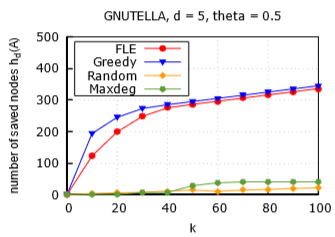
\includegraphics[height = 4.4cm]{picture/FLE/gnu_res} &
		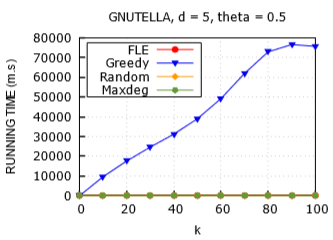
\includegraphics[height = 4.4cm]{picture/FLE/gnu_time} 
		\\
		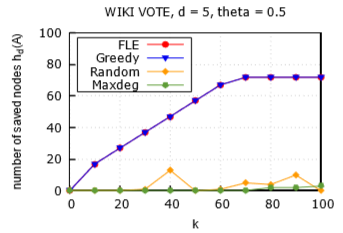
\includegraphics[height = 4.4cm]{picture/FLE/wiki_res} &
		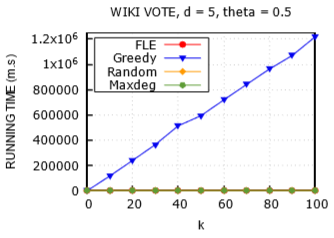
\includegraphics[height = 4.4cm]{picture/FLE/wiki_time} 
		\\
		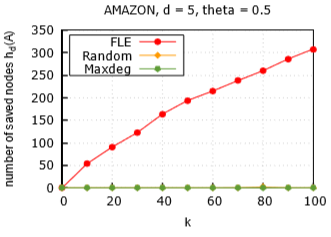
\includegraphics[height = 4.4cm]{picture/FLE/amazon_res} &
		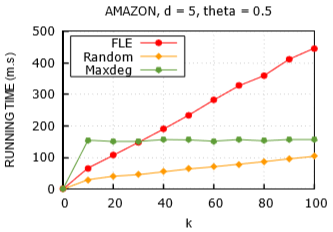
\includegraphics[height = 4.4cm]{picture/FLE/amazon_time} 
		\\
		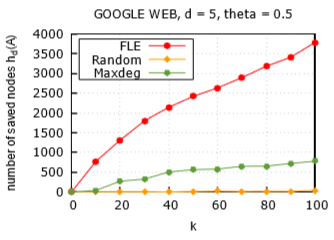
\includegraphics[height = 4.4cm]{picture/FLE/google_res} &
		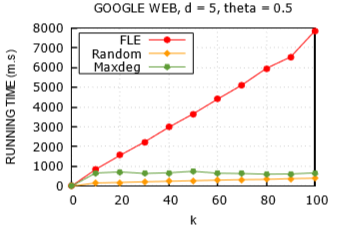
\includegraphics[height = 4.4cm]{picture/FLE/google_time} 
	\end{tabular}
	\caption{So sách chất lượng lời giải và thời gian chạy của các thuật toán khi $k$ thay đổi, $d=5$, $\theta=0.5$.} 
	\label{fig:FLE_k}   
\end{figure}

\begin{figure}[H]
	\begin{tabular}{lll}
		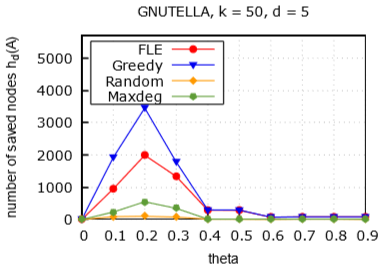
\includegraphics[height = 4.4cm]{picture/FLE/gnu_res_theta} &
		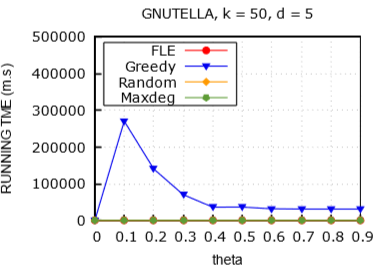
\includegraphics[height = 4.4cm]{picture/FLE/gnu_time_theta} 
		\\
		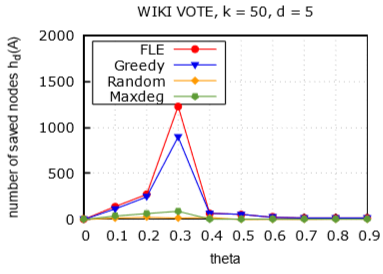
\includegraphics[height = 4.4cm]{picture/FLE/wiki_res_theta} &
		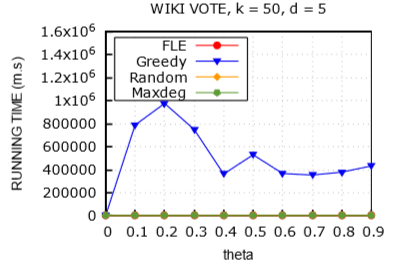
\includegraphics[height = 4.4cm]{picture/FLE/wiki_time_theta} 
		\\
		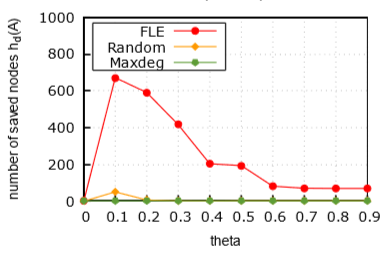
\includegraphics[height = 4.4cm]{picture/FLE/amazon_res_theta} &
		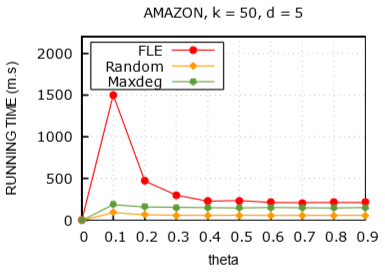
\includegraphics[height = 4.4cm]{picture/FLE/amazon_time_theta} 
		\\
		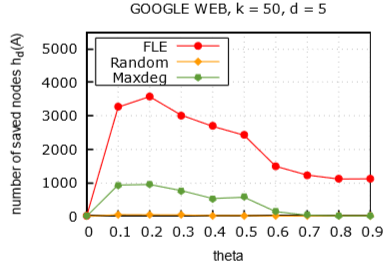
\includegraphics[height = 4.4cm]{picture/FLE/google_res_theta} &
		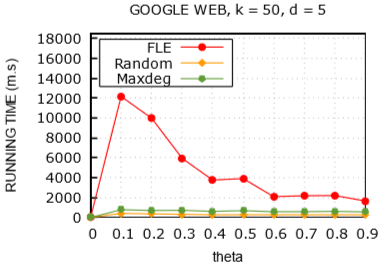
\includegraphics[height = 4.4cm]{picture/FLE/google_time_theta} 
	\end{tabular}
	\caption{So sách chất lượng lời giải và thời gian chạy của các thuật toán khi $\theta$ thay đổi, $d=5$, $k=50$.} 
	\label{fig:FLE_theta}   
\end{figure} 

\begin{figure}[H]
	\begin{tabular}{lll}
		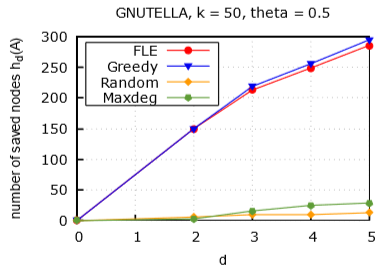
\includegraphics[height = 4.4cm]{picture/FLE/gnu_res_d} &
		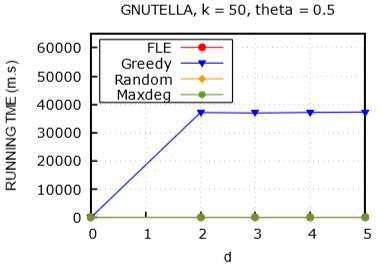
\includegraphics[height = 4.4cm]{picture/FLE/gnu_time_d}
	\end{tabular}
	\caption{So sách chất lượng lời giải và thời gian chạy của các thuật toán khi $d$ thay đổi, $\theta=0.5$, $k=50$ trong mạng Gnutella.} 
	\label{fig:FLE_d}   
\end{figure} 

\section{Bài toán 2: Tìm chi phí nhỏ nhất để ngăn chặn thông tin sai lệch}

Với cách tiếp cận như cách Twitter đã làm năm 2016 là loại bỏ 125.000 tài khoản được nghi ngờ có liên quan đến các hoạt động khủng bố, hay cách tiếp cận như Facebook đã xóa 30.000 tài khoản giả mạo lan truyền các tin đồn trước cuộc bầu cử tổng thống Pháp năm 2017, bài toán Targeted Misinformation Blocking được đưa ra nghiên cứu nhằm mục đích tìm giải pháp xác định được những tài khoản cần loại bỏ khỏi mạng để hạn chế sự phát tán thông tin sai lệch một cách tối ưu nhất.

\subsection{Tổng quan bài tóan}
Nguồn phát tán thông tin sai lệch có thể được phát hiện qua các phương pháp khảo sát, khai phá dữ liệu \cite{qazvin, kwon} và được biểu diễn dưới dạng là tập hợp các đỉnh. Theo các nghiên cứu mới đây \cite{khali, tong, pra}, chiến thuật hiệu quả trong việc ngăn chặn phát tán thông tin sai lệch là xóa bỏ đỉnh hoặc cạnh có vai trò quan trọng trong việc lan truyền thông tin sai lệch. Song tính khả thi của các nghiên cứu trước đây lại bị hạn chế bởi một số khía cạnh sau đây. Thứ nhất họ tập trung vào việc ngăn ngừa thông tin sai lệch bằng nguồn ngân sách hạn chế. Điều này rõ ràng là không thực tế bởi chúng ta khó có thể xác định được bao nhiêu ngân sách cho đủ để ngăn chặn sự lây lan sao cho hiệu quả. Thứ hai, để đảm bảo độ tin cậy của mạng xã hội, chúng ta cần có một biện pháp khử nhiễm thông tin sai lệch với một ngưỡng cho trước, như tỉ lệ giữa người dùng bị nhiễm và người dùng được khử nhiễm. Do đó bài toán này được đưa ra với tính thực tế cao hơn đó là: Dùng ít ngân sách nhất sao cho số lượng người dùng được khử nhiễm lớn hơn một ngưỡng cho trước. Giải pháp đưa ra nhằm tìm một tập đỉnh có ít phần tử nhất để loại bỏ khỏi đồ thị để sao cho nguồn phát tán thông tin sai lêch không thể lan truyền tới được ít nhất ngưỡng $\gamma$ đỉnh yêu cầu. Tổng quan về giải pháp chúng tôi được tóm lược như sau:
\begin{itemize}
	\item Đầu tiên chúng tôi định nghĩa bài toán Xác định và ngăn chặn thông tin sai lệch (Targeted Misinformation Blocking - TMB). Và sau đó chứng minh bài toán TMB có độ khó là $\#P-\text{khó}$.
	\item Với hàm mục tiêu chúng tôi chứng minh nó là hàm submodular và monotone. Trên cơ sở đó, đề xuất một thuật toán tham lam với với tỉ lệ $1+ln(\gamma/\epsilon)$. Song do những hạn chế của thuật toán tham lam, chúng tôi xây dựng thuật toán Scalable $\mathsf{TMB}$ for LT model Algorithm ($\mathsf{STMB}$) để giải quyết cho bài toán TMB với những dữ liệu lớn hơn. 
	\item Việc thực nghiệm được triển khai trên các bộ dữ liệu có sẵn thu thập từ nguồn uy tín và một bộ dữ liệu được chúng tôi thu thập từ mạng xã hội Facebook. 
\end{itemize}

\subsection{Mô hình lan truyền thông tin Ngưỡng tuyến tính Linear Threshold}
Bài toán này sử dụng mô hình lan truyền thông tin Ngưỡng tuyến tính Linear Threshold. Mô hình lan truyền này là mô hình phổ biến, thường được sử dụng trong các nghiên cứu về mạng xã hội. Chi tiết về mô hình LT đã được trình bày trong chương \ref{chap:2}, ta có thể tóm gọn quá trình lan truyền thông tin trên mô hình LT như sau:

Trong mô hình LT, mỗi đỉnh $v \in V$, có hai trạng thái active và inactive. Quá trình lan truyền trên mô hình LT được diễn tả như sau: Đầu tiên, mỗi đỉnh v được gán một trọng số ngẫu nhiên $\theta_{v} \in [0,1]$ thể hiện giá trị active của đỉnh kề u phải đạt được để có thể active v. Tiếp đến quá trình lan truyền diễn ra trong các vòng t = 1,2,3… như sau: 		
\begin {itemize}
\item Ở vòng 1, tất cả các đỉnh $s_{i} \in S$ ở trạng thái active và các đỉnh còn lại ở trạng thái inactive.

\item Ở vòng t $\ge$ 1, một đỉnh v ở trạng thái inactive được active nếu thỏa mãn điều kiện $$\sum_{\mbox{ $u \in N_{in}(v) $ và  u  là active}} w(u, v)\geq \theta_v$$

\item Khi một đỉnh ở trạng thái active thì sẽ luôn duy trì trạng thái đó trong suốt quá trình lan truyền thông tin. Quá trình lan truyền kết thúc khi không có đỉnh nào được active thêm.	
\end {itemize}

\subsection{Định nghĩa bài toán}
Kí hiệu $G = (V, E, w)$ là một đồ thị có hướng biểu diễn cho một mạng xã hội trên mô hình $LT$ với $V$ biểu diễn tập người dùng, $E$ biểu diễn mối quan hệ giữa các cặp người người dùng, $w$ là tập trọng số của các cạnh biểu diễn tần số tương tác giữa các người dùng. Gọi $N_{out}(v)$ và $N_{in}(v)$ lần lượt là tập đỉnh đi ra từ $v$ và đi vào $v$. Mỗi cạnh có hướng $(u,v) \in E$ được gán một trọng số $w(u,v) \in [0,1]$ đảm bảo điều kiện $\sum_{u \in N_{in}(v)} \leq 1$.

Đưa ra một tập nguồn $S = {s_{1}, s_{2}, ... , s_{n}}$, $s_{i} \in V$ là tập tiềm năng phát tán thông tin sai lệch (tương tự như tập hạt giống trong bài IM \cite{kemple2}).

Kí hiệu $\sigma_{S}(G)$ là ảnh hưởng lan truyền của tập S trên đồ thị G dưới mô hình LT hay là số lượng đỉnh được active bởi nguồn S. Theo nghiên cứu của Kempe và các cộng sự \cite{kemple1} đã chỉ ra rằng mô hình LT là tương đương với khả năng tiếp cận trong một đồ thị ngẫu nhiên g, thường được gọi là đồ thị live-edge hoặc đồ thị mẫu. Trên mô hình LT, đồ thị live-edge được xây dựng như sau:
\begin {itemize}
\item Với mỗi v $\in$ V, chọn tối đa một cạnh đi vào nó một cách ngẫu nhiên, xác suất cạnh (u, v) được chọn là w(u, v).

\item Xác suất không có cạnh nào được chọn là 1 - $\sum_{u \in N_{in}(v)} w(u,v)$.
\end {itemize}

Cạnh được chọn gọi là cạnh sống (live-edge) và tất cả các cạnh khác gọi là cạnh bị chặn (blocked-edge). Chúng ta có xác suất tạo ra một đồ thị live-egde g từ G là:
\begin{align}
\Pr[g|G]=\prod_{v \in V}{p(v,g,G)}
\end{align}
với
\begin{equation}
p(v, g, G)= \left\{ \begin{array}{ll}
w(u, v), & \mbox{Nếu $\exists u: (u, v) \in E_g$}\\
1-\sum_{u:(u, v) \in E}{w(u, v)}, & \mbox{Trường hợp khác}\\
\end{array} \right.
\end{equation}

Ảnh hưởng lan truyền của nguồn S khi xóa bỏ các đỉnh trong tập A trên đồ thị G[V$\backslash$A] kí hiệu là $\sigma_{S}(G \backslash A)$. Với A = $\emptyset$, trong \cite{kemple1} đã chỉ ra ảnh hưởng lan truyền của tập nguồn S trên G được tính bởi công thức:
\begin{align}
\sigma_S(G)=\sum_{g \in X_G}{\Pr[g|G]|R(g, S)|}
\label{inf_cal}
\end{align}
trong đó $R(g, S)$ là tập các đỉnh đến được từ S trên g và $X_G$ là tập tất cả các đồ thị live-edge được tạo ra từ G. Đặc biệt, ảnh hưởng lan truyền của tập $S$ có thể được tính bằng đường đi đơn bắt đầu từ $u \in S$ theo công thức: 
\begin{align}
\sigma_{S}(G)=\sum_{x \in \mathsf{P}(G, S)} \prod_{e \in x}w(e)
\label{inf_path}
\end{align} 				
với $\mathsf{P}(G, S)$ là tập tất cả các đường đi đơn từ $s \in S$ tới bất kỳ đỉnh $v \in G \setminus \{S \cup \{s\} \} $ trên đồ thị $G$.		

\textbf{Phát biểu bài toán (Bài toán TMB):} Gọi $G(V,E,w)$ là một đồ thị có hướng biểu diễn một mạng xã hội. Đưa ra một tập nguồn $S = {s_{1}, s_{2}, ... , s_{k}}, S \in V$ là tập tiềm năng phát tán thông tin sai lệch và một số nguyên $\gamma \leq | V |$ thể hiện cho số lượng người dùng tối thiểu chúng ta muốn đảm bảo thông tin sai lệch không lan truyền đến được họ.

\textbf{Yêu cầu:} Tìm tập đỉnh A $\in V \backslash S$ có ít đỉnh nhất sao cho khi xóa các đỉnh trong tập A khỏi đồ thị $G$ thì đảm bảo h(A) = $\sigma_{S}(G) - \sigma_{S}(G \backslash A) \geq \gamma$, tức là đảm bảo ít nhất $\gamma$ người dùng không tiếp xúc với thông tin sai lệch.
\subsection{Độ phức tạp của bài toán}		
Trong mục này chúng tôi chỉ ra một số kết quả về độ khó của bài toán TMB trên mô hình LT.
\begin{theo}
	Cho nguồn tiềm năng phát tán thông tin sai lệch S dưới mô hình LT, bài toán TMB là $\#P-\text{khó}$ nếu S chỉ chứa 1 đỉnh.
\end{theo}
\begin{proof}
	Để chứng minh TMB là $\#P-\text{khó}$ chúng tôi sẽ chỉ ra độ khó của bài toán TMB là lớn hơn hoặc bằng với độ khó của bài toán $s$-$t$ paths mà đã được chứng minh trong \cite{vali} là có độ khó $\#P-\text{khó}$. 
	\begin{define}[Bài toán $s$-$t$ paths \cite{vali}]
		Cho một đồ thị có hướng $G = (V, E), |V| = n, |E| = m$, bài toán $s$-$t$ paths yêu cầu tìm số đường đi có hướng từ đỉnh $s$ tới đỉnh $t$ mà đi qua mọi đỉnh nhiều nhất một lần. 
	\end{define}			
	\begin{figure}[H]
		\begin{center}
			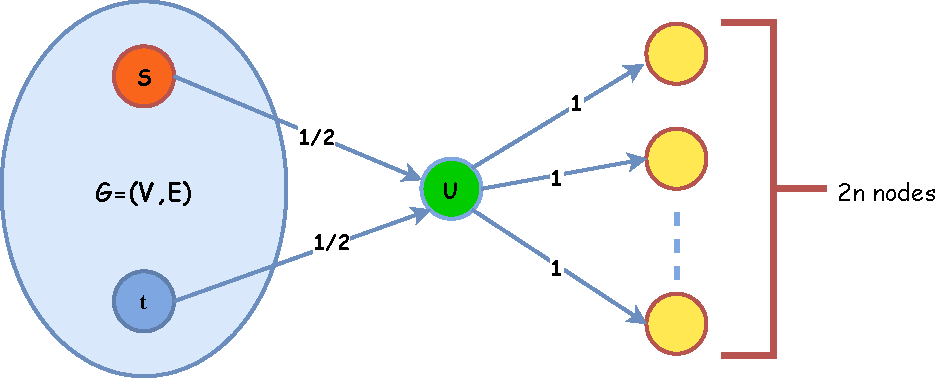
\includegraphics[height = 3 cm]{picture/reduce}
			\caption{Giản thể từ bài toán $s$-$t$ paths sang bài toán TMB.}
			\label{reduce}   
		\end{center}
	\end{figure}			
	Xem xét thể hiện $\mathcal{I}_1$ của bài toán $s$-$t$ paths, với $G = (V, E), s, t$ cho trước. Như minh họa trong hình \ref{reduce}, từ $G$, chúng ta xây dựng $G'$ như sau: Thêm đỉnh u và hai cạnh (s, u), (t, u) với trọng số $w(s, u) = w(t,u) = 1/2$, tiếp đó thêm tập $Q$ gồm 2n đỉnh và kết nối u với chúng với trọng số là 1. Với các cạnh khác, thiết lập trọng số $w = 1/\Delta$, trong đó $\Delta$ là bậc vào lớn nhất của đồ thị $G$. Chúng ta chia tất cả các đường đi bắt đầu từ $s$ thành 2 nhóm: Nhóm thứ nhất là tập tất cả các đường đi có đỉnh kết thúc thuộc tập $\mathcal{Q}$ và nhóm thứ hai là tập còn lại. Từ công thức \eqref{inf_path}, chúng ta có: 
	\begin{align}
	\sigma_{S}(G')&=\sum_{x \in \mathsf{P}(G', s)} \prod_{e \in x}w(e)= \sum_{v \in  G' \setminus Q} \left(  \sum_{x \in \mathsf{P}(G', s, v)} \prod_{e \in x}w(e) \right) + \sum_{v \in Q} \left(  \sum_{x \in \mathsf{P}(G', s, v)} \prod_{e \in x}w(e) \right)  \nonumber
	\\
	&  =\sum_{x \in \mathsf{P}(G, s)} \prod_{e \in x}w(e) + \sum_{x \in \mathsf{P}(G', s, u)} \prod_{e \in x}w(e) + \sum_{v \in   Q } \left(  \sum_{x \in \mathsf{P}(G', s, v)} \prod_{e \in x}w(e)  \right)  \nonumber
	\\
	& = \sigma_{S}(G) +  \sum_{x \in \mathsf{P}(G', s, u)} \prod_{e \in x}w(e) +  \sum_{v \in Q } \left(  \sum_{x \in \mathsf{P}(G', s, v)} \prod_{e \in x}w(e)  \right) 
	\label{eq_1}
	\end{align}  
	và, 
	\begin{align}
	\sum_{v \in  Q } \left(  \sum_{x \in \mathsf{P}(G', s, v)} \prod_{e \in x}w(e)  \right) &= \sum_{v \in Q} \left(  \sum_{x \in \mathsf{P}(G', s, u)} w(u, v)  \prod_{e \in x}w(e)  \right) \nonumber
	\\
	& =\sum_{v \in Q} \left(  \sum_{x \in \mathsf{P}(G', s, u)} \prod_{e \in x}w(e)  \right)\ \ \ \mbox{(Vì $w(u, v)=1$)} \nonumber
	\\
	& = 2n \cdot \sum_{x \in \mathsf{P}(G', s, u)} \prod_{e \in x}w(e)
	\label{eq_3}
	\end{align}
	Từ \eqref{eq_1} và \eqref{eq_3}, chúng ta thu được:
	\begin{align}
	h(u)&= \sigma_{S}(G')- \sigma_{S}(G'\setminus \{u\})=  \sigma_{S}(G')- \sigma_{S}(G)=(2n+1)\cdot \sum_{x \in \mathsf{P}(G', s, u)} \prod_{e \in x}w(e)
	\\
	& = (2n+1)\cdot \left(  w(s, u)+ \sum_{x \in \mathsf{P}(G, s, t)} w(t, u) \prod_{e \in x}w(e) \right) 
	\\
	& = (2n+1)\cdot \left(  \frac{1}{2}+ \frac{1}{2} \sum_{x \in \mathsf{P}(G, s, t)}  \prod_{e \in x}w(e) \right)  \ \ \ \mbox{(Vì $w(s, u)= w(t, u)=\frac{1}{2}$)}
	\\
	& = \frac{2n+1}{2} \left(  \sum_{x \in \mathsf{P}(G, s, t)}  \prod_{e \in x}w(e) +1 \right) 
	\\
	& = \frac{2n+1}{2} \left(  \sum_{i=0}^{n-1} \alpha_i w^i +1 \right) 
	\end{align}   		
	với $\alpha_i=|\mathsf{P}_i(G, s, t)|$. Đặt $f(w)=\sum_{i=0}^{n-1}\alpha_i w^i$. Từ cấu trúc liên kết của G', chúng ta thấy rằng $h(u)=\max_{v \in G'}h(v)$ và $0 \leq  f(w) < 1$. Nếu có thể xác định $f(u) \geq \beta$ với $\forall \beta \in [0, 1]$ trong thời gian đa thức thì chúng ta sẽ giải được bài toán $s$-$t$ paths trong thời gian đa thức. Sử dụng tìm kiếm nhị phân trên đoạn [1, $\Delta^{n-1}$] chúng ta có thể xác định được giá trị của $f(w)$. Yêu cầu này được thực hiện trong $\mathcal{O}(\log(\Delta^{n-1}))=\mathcal{O}((n-1)\log\Delta) =\mathcal{O}(n\log n)$. Do đó việc tính toán $f(u)$ có thể thực hiện trong thời gian đa thức. Tiếp đến thay đổi trọng số w thành n giá trị phân biệt $\frac{1}{\Delta}, \frac{1}{\Delta+1}, \ldots, \frac{1}{\Delta+n-1}$, với mỗi giá trị w áp dụng phương pháp trên chúng ta thu được giá trị $f(w)$ tương ứng. Từ đó có được n phương trình $\sum_{i=0}^{n-1}\alpha_i w^i =f(w), w \in \{\frac{1}{\Delta}, \frac{1}{\Delta+1}, \ldots, \frac{1}{\Delta+n-1} \}$ với $\{\alpha_0, \alpha_2, \ldots, \alpha_{n-1}\}$ là các biến số. Ma trận tương ứng với hệ n phương trình trên là $M_{n \times n}=\{m_{ij}\}$ and $m_{ij}=w^{i} , i,j=0,..,n-1$, dễ thấy đây là ma trận Vandermonde do đó có thể dễ dàng tìm được lời giải $\{\alpha_0, \alpha_2, \ldots, \alpha_{n-1}\}$. Tổng số $s$-$t$ paths trên đồ thị G là $\sum_{i=0}^{n-1} \alpha_i$. Vì thế, nếu chúng ta xác định được $f(u) \geq \beta$ với bất kì $\beta \in [0, 1]$ trong thời gian đa thức thì sẽ giải được bài toán $s$-$t$ paths trong thời gian đa thức. 
	
	Bây giờ, xét thể hiện $\mathcal{I}_2$ của bài toán TMB trong đó $S=\{s\}$, $\gamma = \frac{2n+1}{2}(\beta+ 1) , \beta \in [0, 1]$.  Giả sử rằng $\mathcal{A}$ là một thuật toán giải quyết bài toán TMB trong thời gian đa thức. Xem xét 2 trường hợp: (1) Nếu $\mathcal{A}$ trả ra kết quả là tập $A$ có $|A|=1$, thì chúng ta chỉ cần chọn $A={u}$. Kết luận $f(w) \geq \beta$; (2) Nếu $\mathcal{A}$ trả ra kết quả tập $A$ có $|A| \ge 1$ thì ngoài $u$ sẽ cần chọn thêm một số đỉnh khác. Kết luận $f(w) < \beta$. Vì vậy $\mathcal{A}$ có thể được sử dụng để so sánh $f(w)$ với $\beta$ và có thể giải quyết bài toán $s$-$t$ paths. Điều này chỉ ra rằng bài toán TMB là khó hơn hoặc bằng bài toán $s$-$t$ paths.
\end{proof}
\subsection{Thuật toán đề xuất}
\subsubsection{Thuật toán tham lam (Greedy algorithm)}
Trong phần này chúng tôi giới thiệu một thuật toán xấp xỉ đảm bảo tỉ lệ 1 + ln($\gamma / \varepsilon$) dựa vào tính chất submodular và tính monotone của hàm h($\cdot$). Hàm $f(x)$ được gọi là hàm submodular nếu $A \subset T, v \notin T$ $ f(A+ \{v\})- f(A) \geq f(T+ \{v\})- f(T)$. Còn $f(x)$ được gọi là monotone nếu $\forall T \subseteq S$ chúng ta có $f(T) \leq f(S)$.
\\
\\
\begin{algorithm}[H]			
	\KwData{Graph $G=(V,E, w)$,  $S=\{s_1, s_2, .., s_k\}$, threshold $\gamma < |V|$, parameter $\epsilon \in (0, \gamma)$} 
	\KwResult{set of nodes $A$}
	$A \leftarrow \emptyset$;
	\\
	\While{$h(A) < \gamma-\epsilon $}
	{ 	
		$u=\arg \max_{v \in V\setminus \{A \cup S\}} {h(A+ \{v\})- h(A)}$; 
		\\
		$A \leftarrow A \cup \{u\}$;
	}
	\Return $A$;
	\caption{Greedy Algorithm (GA)}
	\label{GA}
\end{algorithm}
\begin{theo}					
	Hàm $h(\cdot)$ là hàm submodular và monotone. 
	\label{sub}
\end{theo}	

\begin{proof}	
	Theo định lý 5 trong \cite{khali}, cho $A \subseteq T$ chúng ta có $h(T)-h(A)=\sigma_S(G) - \sigma_S(G \setminus T) -(\sigma_S(G) - \sigma_S(G \setminus A))  =\sigma_{S}(G \setminus A)- \sigma_{S}(G \setminus T) \geq 0$. Do đó $h(\cdot)$ là một hàm monotone. 
	
	Tiếp đến chúng ta chỉ ra rằng $\sigma_S(G \setminus A)$ là một hàm submodular với $A$ là biến số. Kí hiệu $N_E(A)$ là tập tất cả các cạnh (u, v) $\in$ E với u, v $\in$ $A$. Đặt $E_{T, v}=N_E(T+\{v\})\setminus N_E(T), E_{A, v}= N_E(A+\{v\}) \setminus N_E(A)$ dễ thấy $E_{T, v} \subseteq E_{A, v}$  nếu $A \subseteq T$ $\Rightarrow$ $N_E(A)\cup E_{T, v} \subseteq N_E(A+ \{v\})$. Lấy $\sigma_S(G \setminus N_E(X))$ là ảnh hưởng lan truyền của tập $S$ trên đồ thị $G$ sau khi loại bỏ tập cạnh $N_E(X) \subset E$, chúng ta nhận thấy $\sigma_{S}(G \setminus X)=\sigma_{S}(G \setminus N_E(X)$. Theo định lý 6 trong \cite{khali}, $\forall N_E(X) \subseteq N_E(Y), e \in N_E(Y)\setminus N_E(X)$, chúng ta có: 
	\begin{align}
	\sigma_{S}(G \setminus (N_E(X) \cup \{e\}) - \sigma_{S}(G \setminus X) 
	\leq \sigma_{S}(G \setminus (N_E(Y) \cup \{e\})) - \sigma_{S}(G \setminus Y)
	\label{super}
	\end{align}
	Vì thế,
	\begin{align}
	\sigma_{S}(G \setminus A)-\sigma_{S}(G \setminus (A \cup \{v\})) 
	& =\sigma_{S}(G \setminus N_E(A))-\sigma_{S}(G \setminus N_E(A+\{v\})) 
	\\
	&	\geq \sigma_{S}(G \setminus N_E(A))-\sigma_{S}(G \setminus (N_E(A) \cup E_{T, v})) 
	\\
	&	\geq \sigma_{S}(G \setminus N_E(T))-\sigma_{S}(G \setminus (N_E(T) \cup E_{T, v}))  
	\\
	& = \sigma_{S}(G\setminus T)-\sigma_{S}(G \setminus (T \cup \{u\}))  (\mbox{Theo BĐT \eqref{super}})
	\end{align}
	Kết hợp với công thức $h(A)= \sigma_S(G)- \sigma_S(G\setminus A)$ chúng ta có được $h(\cdot)$ là một hàm submodular.
\end{proof}

\begin{theo} Với $\forall$ $\epsilon \in (0, \gamma)$, thuật toán \ref{GA} đưa ra lời giải $A$ thỏa mãn $h(A) \geq \gamma- \epsilon$, và $|A|$ là không vượt quá tích của $1+\ln(\gamma/ \epsilon)$ với số đỉnh của lời giải tối ưu \label{app}
\end{theo}		
\begin{proof}
	Chi tiết cách chứng minh định lý \ref{app} được chỉ ra trong \cite{snam}. 
\end{proof}
Thuật toán tham lam có cách tiếp cận khá đơn giản là mỗi bước tìm đỉnh $u$ sao cho hàm $h(A)$ tăng nhiều nhất. Song vấn đề khó khăn nhất gặp phải là tính giá trị hàm $\sigma(\cdot)$ có độ khó là $\#P-\text{khó}$, chứng minh trong \cite{vali}. Vì vậy chúng tôi đưa ra một thuật toán hiệu quả trong phần sau.

\subsubsection{Thuật toán STMB (STMB algorithm)}
Thuật toán tham lam đưa ra một lời giải tốt xong lại không đảm bảo yêu cầu về thời gian với dữ liệu lớn do đó trong phần này chúng tôi đưa ra một giải pháp đảm bảo yêu cầu cả về chất lượng lời giải cũng như thời gian tính toán. Dưới đây là các bước chính trong thuật toán chúng tôi đề xuất:
\begin {itemize}
\item Đầu tiên sáp nhập các đỉnh trong tập nguồn S thành một nút I bằng cách áp dụng thuật toán \ref{MERGE} được đề xuất bởi Zhang \cite{yao16}. Chúng ta thu được một đồ thị mới và nguồn phát tán thông tin sai lệch bây giờ chỉ còn là một đỉnh I duy nhất.
\end{itemize}
\begin{algorithm}[H]			
\KwData{Graph $G=(V,E, w)$,  $S=\{s_1, s_2, .., s_k\}$} 
\KwResult{Graph $G'=(V', E', w')$, I}
$G' \leftarrow G$;
\\
Add node I to G'			
\\
\ForEach{s $\in$ S}
{
	\If{$\exists$ (s, v) }
	{
		\eIf{(I, v) $\notin$ G'}
		{
			Add edge (I, v) to G'
			\\
			w'(I, v) = w(s, v)
		}
		{
			w'(I, v) = w'(I, v) + w(s, v)
		}
		Remove (s,v) from G'
	}
}
Remove all node in S from G'
\\
\Return G', I;
\caption{MERGE Algorithm(MERGE)}
\label{MERGE}
\end{algorithm}	
\begin {itemize}			
\item Tiếp đến chúng tôi tạo ra $\mu(\mu \in N*)$ đồ thị mẫu g từ G bằng cách: mỗi đỉnh v $\in$ V chọn nhiều nhất một đỉnh kề đi đến nó một cách ngẫu nhiên sao cho xác suất chọn cạnh (u, v) là w(u, v) và xác suất không chọn cạnh nào là 1 - $\sum_{u} w(u, v)$. Những cạnh được chọn được gọi là cạnh sống  (live - edge) và tất cả các cạnh còn lại được gọi là cạnh bị chặn (blocked-edge). Chi tiết cách lấy đồ thị mẫu được mô tả trong thuật toán \ref{GSGLT} và trong hình \ref{example}: 
\end {itemize}
\begin{figure}[H]
\subfloat[Đồ thị $G'$ sau khi hợp nhất các đỉnh trong nguồn S\label{fig:test1}]
{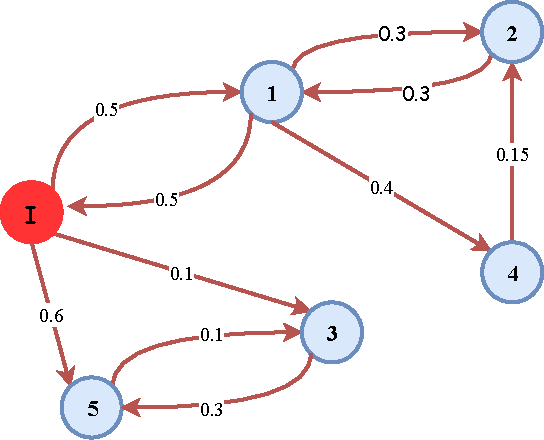
\includegraphics[width=.3\linewidth]{picture/1}}\hfill
\subfloat[Đồ thị mẫu $g$\label{fig:test2}]
{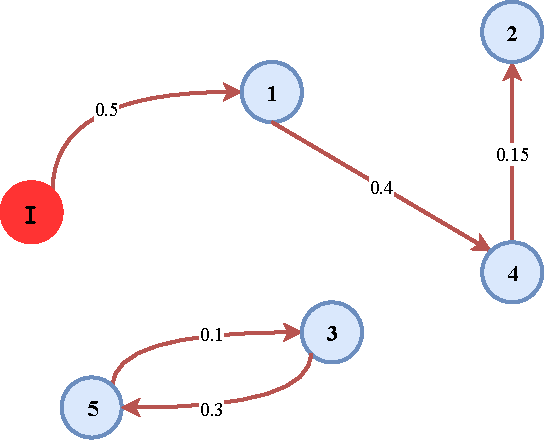
\includegraphics[width=.3\linewidth]{picture/2}}\hfill
\subfloat[Cây gốc $I$ tạo ra từ $g$ \label{fig:test3}]
{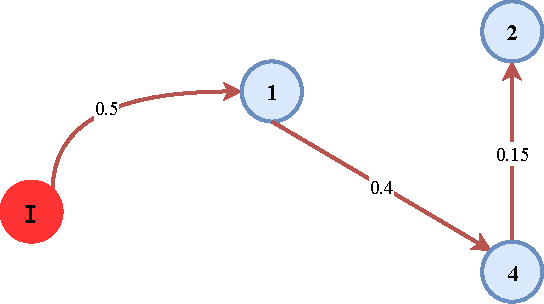
\includegraphics[width=.3\linewidth]{picture/3}}
\caption{Ví dụ tạo ra một cây gốc $I$ từ $G$ trên mô hình LT}
\label{example}
\end{figure}	
\begin{algorithm}[H]
\KwData{Graph G=(V,E, w), I} 
\KwResult{Tree g root at I}			
g $\Leftarrow \emptyset$
\\
\For{$v \in V_G$}
{	
	$\gamma_{active} \leftarrow$ random(0, 1)
	\\
	sum\_weight $\leftarrow$ 0
	\\
	\For{u $\in$ in\_neighbors(v)}
	{
		sum\_weight += w(u, v)
		\\
		\If{sum\_weight $\geq \gamma_{active}$}
		{
			Add edge (u, v) to g
			\\
			Break
		}
	}
}		
g $\leftarrow$ DFS$_{tree}$(I,g)
\\
\Return g
\caption{Get Sample Graph LT Algorithm (GSG\_{LT})}
\label{GSGLT}
\end{algorithm}	
\begin {itemize}
\item Trên cây T$_{I}^i$, ảnh hưởng địa phương của nút v là số nút con của cây gốc v kể cả v trên cây T$_{I}^i$. Áp dụng thuật toán DFS dễ dàng tìm được số nút con của v. Ảnh hưởng giảm của nguồn S khi loại đỉnh u khỏi G bằng lượng ảnh hưởng giảm trung bình khi loại u trên tất cả các cây T$_{I}^i$. Kí hiệu h(u, $T_I^i$) là lượng ảnh hưởng giảm trên cây $T_I^i$ sau khi loại bỏ đỉnh u khỏi $T_I^i$. Áp dụng phương pháp Lazy forward của Leskovec \cite{lazy} để tìm kiếm lời giải. 
\end {itemize}
\begin{algorithm}[H]
%\SetAlgoNlRelativeSize{0}
\KwData{Graph $G=(V,E, w)$,  $\mathcal{S}=\{s_1, s_2, .., s_q\}$, threshold $\gamma>0$} 
\KwResult{set of nodes $A$}
$A \leftarrow \emptyset$;	$(G', I) \leftarrow \mathtt{Merge}(G, \mathcal{S})$.
\\
Remove all node, $I$ can't reach in $G$.
\\
Generate $\eta$ sample graphs and set $\eta$ trees $\mathcal{L}=\{T_{I}^1, T_{I}^2, \ldots, T_{I}^{|\mathcal{\eta}|}\}$
\\
For each $ T_{I} \in \mathcal{L}$, calculate $h(u, T_{I})$ for all $u \in T_{I}$ (by using DFS algorithm).
\\
\For{$u \in V$}
{
	$u.\delta(u) \leftarrow \frac{1}{\eta}\sum_{T_{I} \in \mathcal{L}} h(u, T_{I})$; $u. cur \leftarrow 1$
	\\
	Insert element $u$ into $Q$ with $u.\delta(u)$ as the key
}
$ h_{max} \leftarrow 0$; $iteration \leftarrow 1$
\\
\While{$ h_{max} <\gamma-\epsilon $}
{
	$u_{max} \leftarrow  dequence \  Q$
	\\
	\eIf{$u_{max}.cur =iteration$}
	{
		$A \leftarrow A \cup \{u_{max}\}$ ; $iteration \leftarrow iteration+1 $
		\\
		\ForEach{$T_{I} \in \mathcal{L}_c $}
		{
			If $u_{max} \in T_{I}$, remove node $u_{max}$ and update $h(v, T_{I})$, $ \forall v \in T_{I}$.
		}
		$h_{max} \leftarrow h_{max}+ u_{max}.\delta(u_{max})$
	}
	{
		$u_{max}. \delta(u_{max}) \leftarrow  \frac{1}{\eta}\big(\sum_{T_{I} \in \mathcal{L}}h(I, T_{I}) - \sum_{T_{I} \in \mathcal{L}} h(I, T_{I} \setminus u_{max})\big)$
		\\
		$u_{max}. cur =iteration$; re-insert $u_{max}$ into $Q$
	}
}
\Return $A$;
\caption{Scalable $\mathsf{TMB}$ for LT model ($\mathsf{TMB}$) Algorithm}
\label{STMB}
\end{algorithm}				
{\itshape Độ phức tạp của thuật toán: }		
Để đánh giá độ phức tạp của thuật toán trước tiên chúng ta đi phân tích độ phức tạp của các thuật toán con trong nó.
\begin {itemize}
\item Thuật toán MERGE có độ phức tạp là O(k + | N$_{in}(S)$ |).

\item Quá trình tạo ra $\mu$ đồ thị mẫu dòng 3 có độ phức tạp O($\mu(m + n)$).

\item Do T$_{I}^i$ là một cây nên việc tính toán h(u, T$_{I}^i$) $\forall u \in \text{T}_{I}^i$ mất O$(\mu n)$ 

\item Phần Lazy Forward có độ phức tạp là O(qmn) với q là số vòng lặp từ dòng 10 đến 23.
\end {itemize}

Vậy nên toàn bộ thuật toán TMB có độ phức tạp là O($\mu$(m+qn)).

\subsection{Kết quả thực nghiệm với dữ liệu với dữ liệu có sẵn}	

Trong mục này chúng tôi đưa ra kết quả thực nghiệm của thuật toán STMB với 3 bộ dữ liệu có sẵn của các mạng xã hội và so sánh về chất lượng lời giải, tốc độ thực hiện với một số thuật toán cơ bản khác.
Thuật toán được thực hiện bằng ngôn ngữ Python 2.7, sử dụng thư viện hỗ trợ NetworkX\footnote{Hướng dẫn sử dụng https://networkx.github.io/} và chạy trên máy Linux Server với 2.30 GHz Intel\textsuperscript{\textregistered} Xeon\textsuperscript{\textregistered} CPU E5-2697, bộ nhớ 128G of RAM DDR4.
\subsubsection{Dữ liệu}
Với mục đích thực nghiệm, chúng tôi sử dụng 3 bộ dữ liệu mạng thực tế thu thập trên trang snap.stanford.edu \footnote{https://snap.stanford.edu/data/index.html}, Một vài thông tin cơ bản về chúng được đưa ra trong bảng \ref{TMB:table}. 
\begin{table}[h]
	\centering
	\begin{tabular}{|c|c|c|c|}
		\hline 
		Mạng & NetS & AS & NetHEPT\\ 
		\hline 
		Số đỉnh & 1.5K & 6.4K & 15.2K \\ 
		\hline 
		Số cạnh & 5.4K & 12.5K & 32.2K\\ 
		\hline 
		Bậc trung bình & 3.8 & 7.5 & 4.2\\ 
		\hline 
		Số đỉnh nguồn & 100 & 300 & 1000\\ 
		\hline 
	\end{tabular} 
	\caption{Các bộ dữ liệu dùng trong thực nghiệm với giải pháp TMB}
	\label{TMB:table}
\end{table}

\texttt{NetS}\cite{NetS}: Một mạng lưới các nhà khoa học làm việc trên lý thuyết và thử nghiệm mạng, được biên soạn vào tháng 5/2006.

\texttt{AS}\cite{AS}: Biểu đồ các bộ định tuyến bao gồm Internet có thể được sắp xếp thành các biểu đồ con được gọi là Autonomous Systems(AS). Mỗi AS trao đổi lưu lượng với một số hàng xóm(peer). Chúng ta có thể xây dựng một mạng lưới các AS liên kết với nhau dựa trên nhật ký BGP(Border Gateway Protocol). Bộ dữ liệu là kết quá từ dự án University of Oregon Route Views. 

\texttt{NetHEPT}\cite{kemple1, chen10LT}: Một mạng lưới hợp tác học thuật được trích xuất từ phần "High Energy Physics-Theory" của trang điện tử arXiv\footnote{https://arxiv.org/} trong khoảng thời gian từ năm 1991--2003. Mỗi đỉnh trong mạng đại diện cho một tác giả và mỗi cạnh kết nối 2 đỉnh cho biết 2 tác giả đã đồng tác giả của một bài báo.

\subsubsection{Các thiết lập}
Chúng tôi sử dụng các thiết lập dưới đây cho việc đánh giá thực nghiệm:
Theo các nghiên cứu trước \cite{khali, kemple1,chen10LT}, chúng tôi thiết lập trọng số các cạnh của đồ thị trên mô hình LT theo công thức $w(u,v) = 1/N_{in}(v)$. Với nguồn phát tán thông tin sai lệch chúng tôi chọn ngẫu nhiên từ 4-6\% số lượng đỉnh của cả đồ thị, phụ thuộc vào kích thước của đồ thị. 


\subsubsection{Các thuật toán sử dụng}
Trong thực nghiệm, chúng tôi so sánh thuật toán STMB với một số thuật toán sau:
\begin {itemize}
\item PageRank: Tính toán ranking của các đỉnh trong đồ thị $G$ dựa vào cấu trúc các cạnh liên kết với nó. Đây là thuật toán được thiết kế để xếp hạng các trang web từ đó đưa ra kết quả tìm kiếm. Do $h(\cdot)$ là hàm monotone nên sau khi sắp xếp hạng của các đỉnh trong đồ thị, chúng tôi sử dụng thuật toán tìm kiếm nhị phân để tìm kiếm tập lời giải A với |A| đỉnh có rank lớn nhất.
\item High-Degree: Một thuật toán heuristic dựa vào bậc của một đỉnh. Bậc của một đỉnh ở đây là tổng số đỉnh được tính theo công thức $d(v) = N_{in}(v) + N_{out}(v)$. Tương tự như thuật toán PageRank sau khi sắp xếp các đỉnh dựa trên bậc của chúng, chúng tôi sử dụng thuật toán tìm kiếm nhị phân để tìm lời giải cho bài toán.
\item Greedy: Thuật toán Greedy đưa ra trong thuật toán \ref{GA} kết hợp với các tối ưu trong \cite{Jleskovec} giúp tăng tốc độ thuật toán song không làm ảnh hưởng đến chất lượng lời giải.
\end{itemize} 

\subsubsection{Kết quả thực nghiệm} 
Như mô tả trong hình \ref{solSTMB}, số lượng đỉnh được chọn đưa ra bởi thuật toán STMB là nhỏ nhất. STMB tốt hơn lên đến 39\% so với thuật toán Greedy, hơn 60\%-95\% và 57\%-87\% so với thuật toán PageRank và High-Degree tương ứng. Để kiểm tra kết quả thu được từ thuật toán STMB, chúng tôi chạy 10000 mẫu Monte-Carlo để ước lượng giá trị của hàm $h(A)$ và kết quả kiểm tra được đưa ra trong hình \ref{check}. Trong hầu hết các trường hợp $h(A)$ vượt qua ngưỡng yêu cầu.
\begin{figure}[H]
\begin{tabular}{lll}
	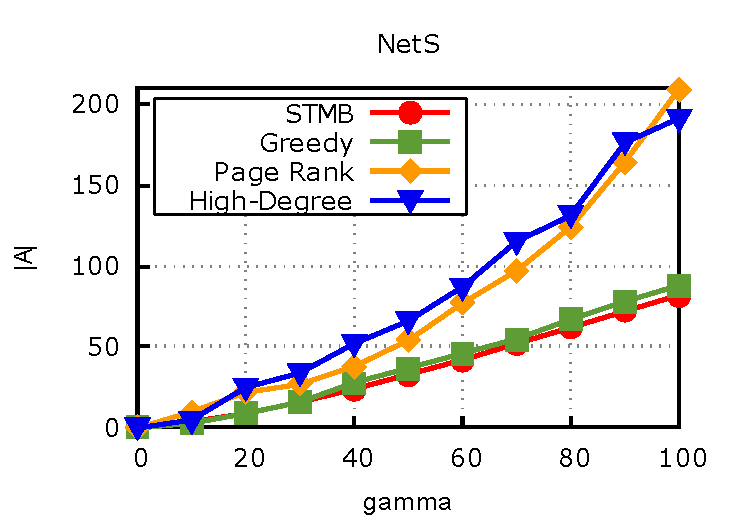
\includegraphics[height = 3.2cm]{picture/NetS} &
	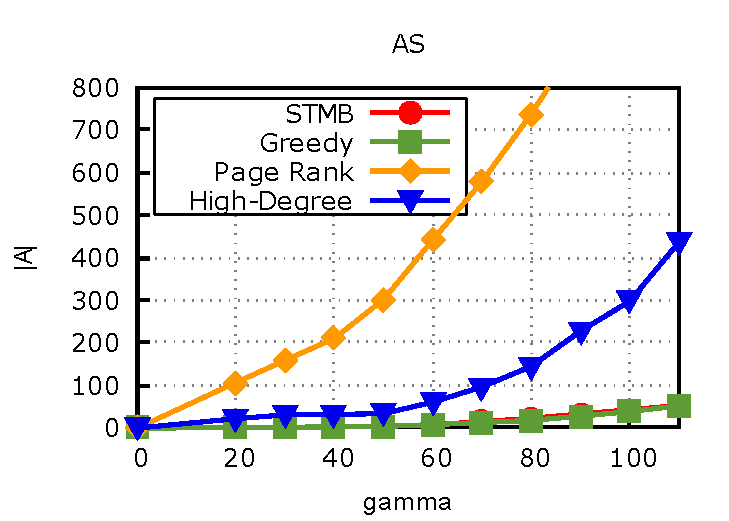
\includegraphics[height = 3.2cm]{picture/AS} &   
	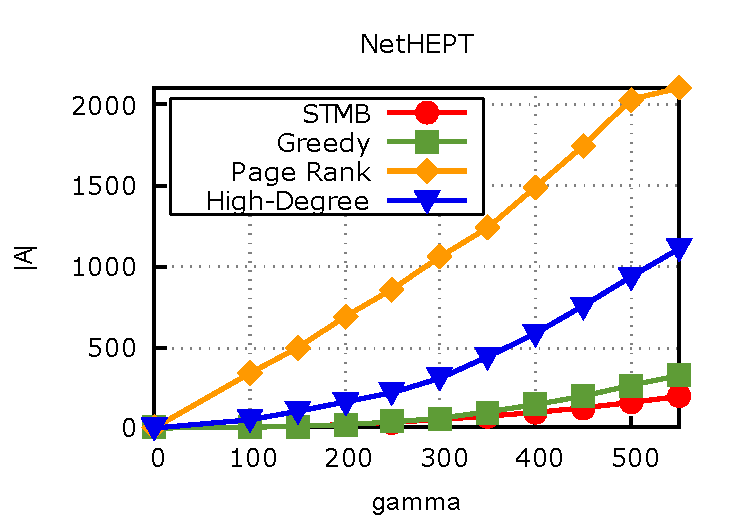
\includegraphics[height = 3.2cm]{picture/NetHEPT}
	\\
	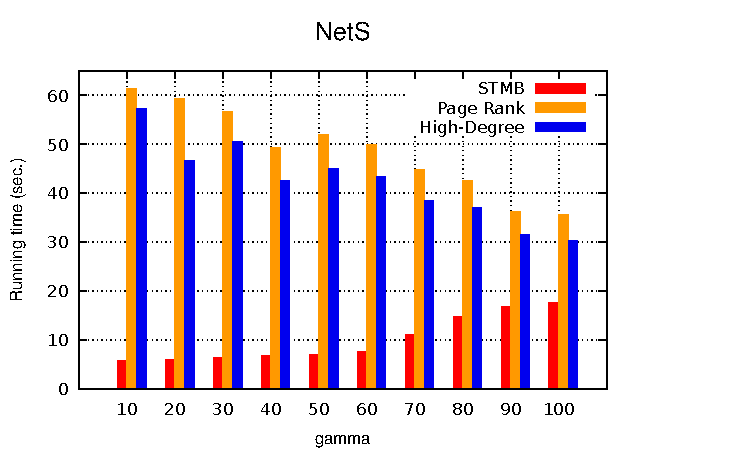
\includegraphics[height = 3.2cm]{picture/TimeNetS} &
	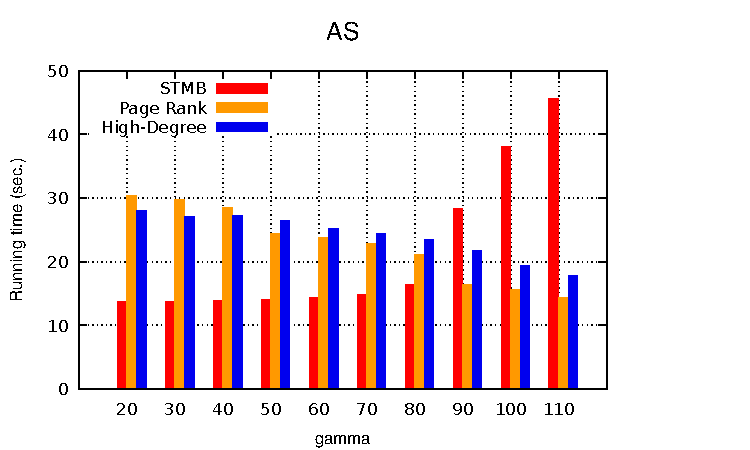
\includegraphics[height = 3.2cm]{picture/TimeAS} &   
	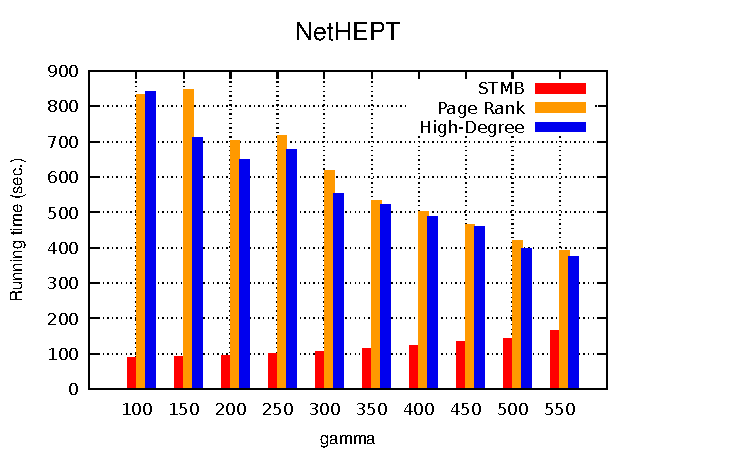
\includegraphics[height = 3.2cm]{picture/TimeNetHEPT}
\end{tabular}
\caption{So sách chất lượng lời giải và thời gian chạy của các thuật toán cho bài toán TMB}
\label{solSTMB}    
\end{figure}
\begin{figure}[H]
\begin{tabular}{ccc}
	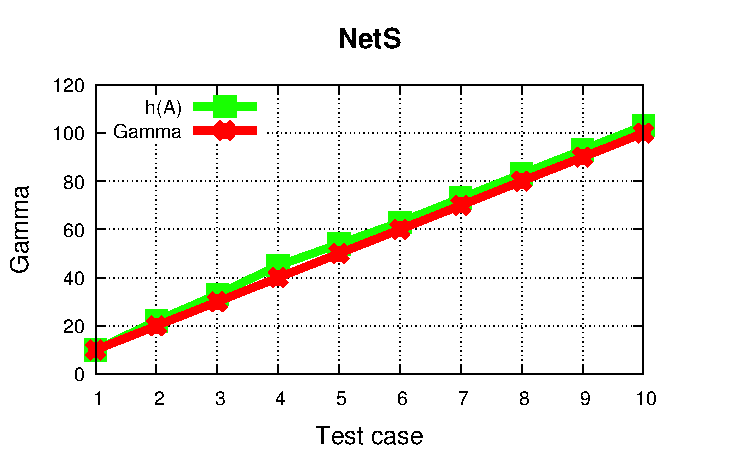
\includegraphics[height = 3.2 cm]{picture/CheckNetS} &
	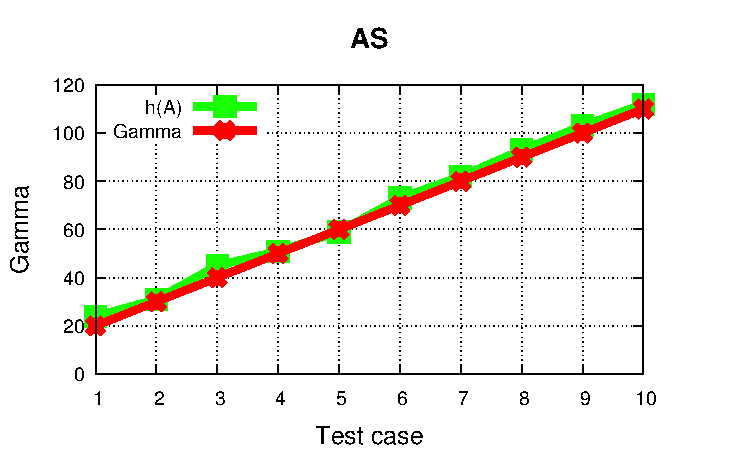
\includegraphics[height = 3.2 cm]{picture/CheckAS} &   
	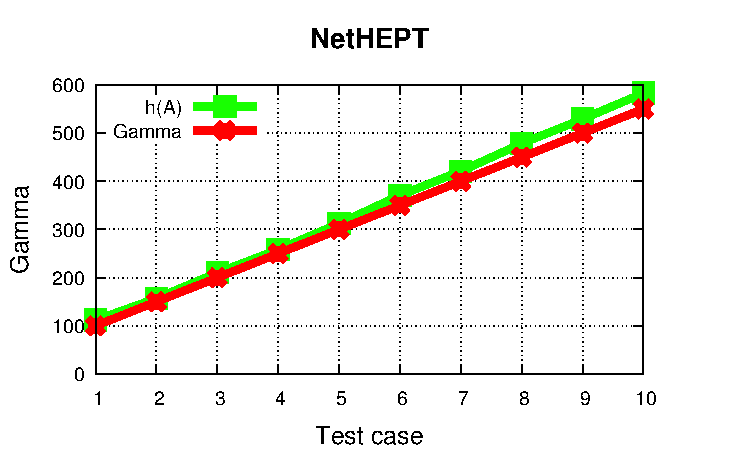
\includegraphics[height = 3.2 cm]{picture/CheckNetHEPT}
\end{tabular}
\caption{Kiểm tra kết quả của thuật toán STMB}
\label{check}    
\end{figure}
\begin{table}[h]
\label{tab:time}       % Give a unique label
% For LaTeX tables use
\begin{center}
	\begin{tabular}{|c|c|c|c|c|}				
		\hline 
		\textbf{} & {$\mathsf{STMB}$} & {$\mathsf{Greedy}$} & {Page Rank} & {High-Degree} 				
		\\ 
		\hline 
		NetS & \textbf{17.57(s)} &	14206.80(s) &	35.73(s) &	30.24(s)
		\\ 
		\hline 
		AS & 45.70(s) & 14074.87(s) & \textbf{14.39(s)} &	17.85(s)
		\\
		\hline 
		NetHEPT & \textbf{165.12(s)} & 582566.74(s) & 392.34(s) & 374.66(s)
		\\
		\hline 
	\end{tabular}
\end{center}
\caption{So sánh thời gian chạy của các thuật toán với trường hợp $\gamma$ lớn nhất}
\label{timeSTMB}
\end{table}
Thời gian chạy của các thuật toán trên 3 bộ dữ liệu trong trường hợp có $\gamma$ là lớn nhất được đưa ra trong bảng \ref{timeSTMB} cho thấy thuật toán Greedy có chất lượng lời giải tương đương với thuật toán STMB song thời gian thực nghiệm trên các bộ dữ liệu lại rất không hiệu quả. Trong khi đó thuật toán STMB có thời gian thực hiện khá là nhanh, không khác biệt nhiều so với các thuật toán cơ bản song vẫn đảm bảo có một lời giải tốt.